\chapter{Introduction}
\label{chapt: intro}

``A pulsar,’’ so goes the traditional paper opening, ``is a highly-magnetised, rapidly-rotating neutron star’’. The first pulsar discovered was CP~1919+21 (now known as PSR~B1919+21 or PSR~J1921+2153) by \citet{HBP+1968} in Cambridge on the 28th November 1967. Appearing as a series of regularly-spaced peaks in radio observations, the signals were quickly associated with emission from the then-theoretical neutron stars \citep{BZxx1934}; extremely compact stellar remnants, with masses of around 1.4 solar masses (M$_\odot$) and radii of approximately 10~km \citep[e.g.][]{PulsarAstronomy}. These properties place neutron stars among the densest objects in the universe with an average density of $\sim$6.7$\times10^{17}$~kg~m$^{-3}$, around three times the density of nuclear matter \citep[$2.3\times10^{17}$~kg~m$^{-3}$; e.g.][]{Lxxx2001}. This density makes the rotation of neutron stars extremely stable, and gives them strong surface gravitational fields. Neutron stars also have incredibly powerful magnetic fields; about $10^{12}$~gauss at the stellar surface \citep{Gxxx1968}.

Pulsars -- ``PULSating stARS'' -- appear in radio frequency time-series observations as a series of regularly-separated peaks. Their radio emission is believed to be produced from around their magnetic axis, which is not necessarily aligned with their rotation axis. As the star rotates, radio beam sweeps round the sky creating an effect that is comparable to a ``cosmic lighthouse''. The inclined magnetic axis causes the pulsar to lose energy through the emission of magnetic dipole radiation, leading to the predication of a gradual decrease in their rotation rates \citep{Pxxx1968}. This was first confirmed by the spin-down of the Crab pulsar (PSR~B0531+21), whose period was observed to increase by 36 ns per day \citep{RCxx1969_crab}.

The presence of a strong magnetic field surrounding a dense, superconducting star causes a pulsar to act as a homopolar or ``Faraday disk'' generator, in which an enormous potential difference is generated between the poles and the equator. For a pulsar where the magnetic and rotation axes are aligned (an ``aligned rotator''), \citet{GJxx1969} calculated that the induced electric fields would lead to streams of electrons being emitted from the poles, and bunches of ions being produced from the equator. These particles form a dense plasma magnetosphere around the star, in which the charged particles co-rotate with the pulsar up until the ``light cylinder'' radius, the distance at which their velocities would have to exceed the speed of light to maintain co-rotation. Later analysis showed that the surface of a neutron star is not hot enough to sustain an outflow of positively-charged ions. \citet{RSxx1975} instead proposed that a model in which electron-positron pairs are produced within a ``polar gap'' close to the surface of the magnetic poles, in which the enormous electric fields are not screened by plasma. The positrons escape from the star along the open magnetic field lines, and to close the homopolar generator circuit the electrons return to the surface of the pulsar.

Radio emission produced by a pulsar is believed to originate from these ultra-relativistic particles streaming from the magnetic poles, at a certain height above the surface of the star. The structure of the emission region is not yet fully understood, and a successful model must explain both the variability of individual pulses, and the stability of the profile integrated over long periods. In the model proposed by \citet{RSxx1975}, the rotating carousel model can explain the time-dependent periodic drift seen in the individual pulses of some pulsars. 

A key aspect of pulsar radio emission is its polarisation. The long-established model which aims to explain the change in linear polarisation angle with pulse phase is the Rotating Vector Model \citep[RVM;][]{RCxx1969}. This is a purely geometric model that suggests that the angle of polarisation depends only on the rotational phase of the pulsar and the observing geometry. However, deviations from this model are commonly seen, for example in the form of discontinuous polarisation angle jumps. These are believed to originate from two modes of emission which are orthogonally polarised, with the observed transition occurring when the dominating mode changes.

This introductory chapter is designed to provide an overview of the properties of radio pulsars, and to introduce the key models and concepts on which the rest of this thesis is based. Section~\ref{sec: intro - general intro} presents the observable spin parameters of pulsars and explains how these may be used to derive other properties. The population is then introduced, and different classes are highlighted in Sec.\ref{sec: intro - general intro - pulsar population}. Section~\ref{sec: intro - emission models} gives a basic overview of how the radio emission is believed to be produced. Pulsar polarisation and models are introduced in Sec.~\ref{sec: intro - emission models - polarisation}, and the variability of single pulses are described in Sec.~\ref{sec: intro - emission models - single pulse phenomena}. Section~\ref{sec: intro - observation processing} describes polarisation and flux calibration of pulsar data and Sec.~\ref{sec: intro - observation processing - ISM effects} explains some of the effects of the interstellar medium on propagating radiation. Finally, Sec.~\ref{sec: intro - thesis outline} gives an outline of the following chapters and results of this thesis.












\section{Properties of radio pulsars}
\label{sec: intro - general intro}

This section introduces the basic properties of radio pulsars which can be measured from their radio pulses. A simple schematic view of the geometry of a pulsar is shown in Fig.~\ref{fig: intro - basic geometry}. The magnetic field at the altitude above the surface of the star where the radio emission is produced is thought to be dominated by the dipole moment. The two main parameters that describe the viewing geometry are the angles $\alpha$ and $\beta$. The magnetic inclination angle $\alpha$ is the angle between the rotation and magnetic axes, and $\beta$ is the impact angle between the magnetic axis and the observer's line of sight (LOS) as the pulsar rotates. 
\begin{figure}
    \begin{center}
        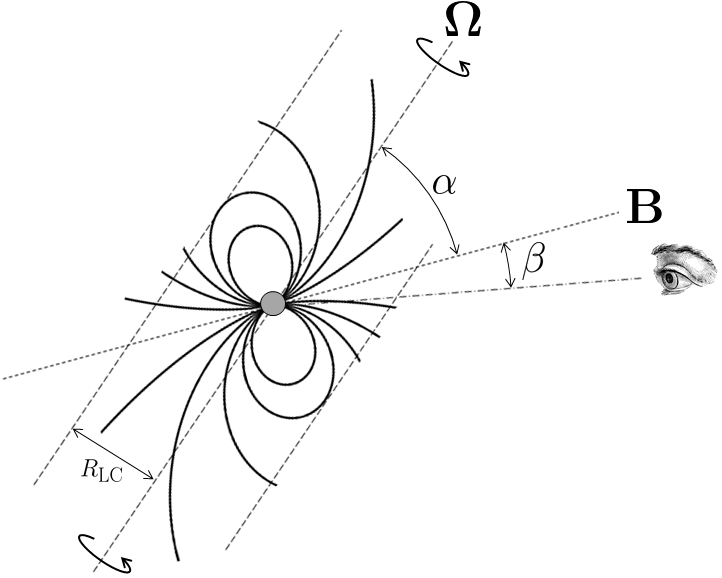
\includegraphics[width=0.75\textwidth]{Figures/Introduction/pulsar_geometry}
        \caption[The basic geometry of a radio pulsar]{The geometry of a pulsar with a dipolar magnetic field ($\mathbf{B}$) inclined at an angle $\alpha$ to the rotation axis ($\mathbf{\Omega}$). The observer's line of sight makes an angle $\beta$ to the magnetic axis. The light cylinder radius $R_\mathrm{LC}$ is the distance at which an object corotating with the pulsar would have speed equal to the speed of light, $c$.}
        \label{fig: intro - basic geometry}
    \end{center}
\end{figure}
Although the magnetosphere co-rotates with the star, co-rotation can only be sustained up to the distance at which a particle would have to move at the speed of light. This defines the ``light cylinder'', which is at a radius $R_\mathrm{LC} = cP/2\pi$, where $c$ is the speed of light and $P$ is the pulsar's rotation period. If a magnetic field line remains within $R_\mathrm{LC}$ it reconnects to the pulsar and is a ``closed'' field line, whereas those that cross the light cylinder are ``open'' field lines and particles with trajectories bound to these can escape the pulsar. At this boundary, the last set of field lines which cross $R_\mathrm{LC}$ are referred to as the ``last open field lines'', and these form the boundary around the ``open field line region'' which contains all field lines which do not close within $R_\mathrm{LC}$

As illustrated in Fig.~\ref{fig: intro - emission cone}, the radio emission is thought to originate from within a cone around the magnetic axis, which is bound by the tangents to the last open field lines at the emission height $h_\mathrm{em}$.  
\begin{figure}
    \begin{center}
        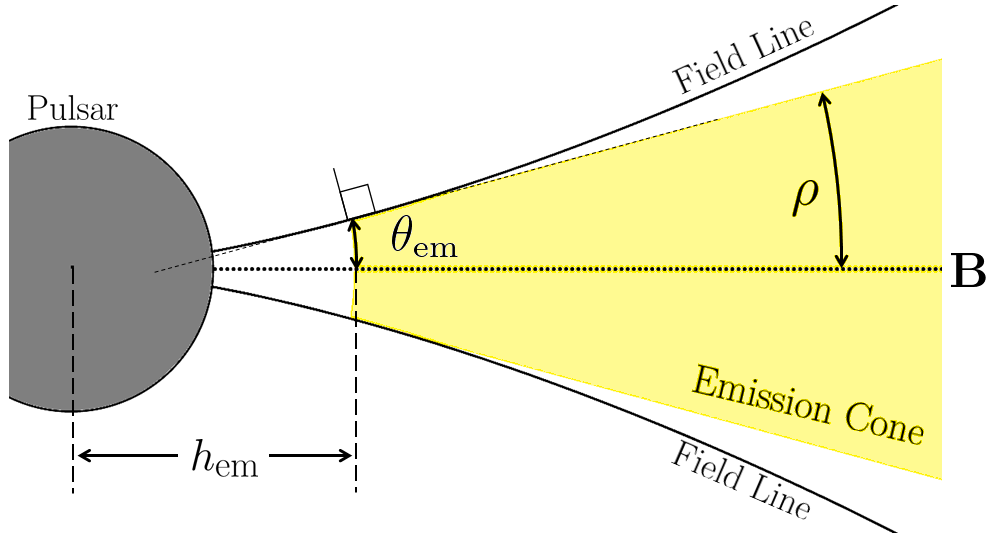
\includegraphics[width=0.75\textwidth]{Figures/Introduction/cone}
        \caption[The geometry of the emission cone]{The cone of emission of half opening angle $\rho$ surrounding the magnetic axis, $\mathbf{B}$. The cone is delimited by tangents to the last open field lines at the emission height $h_\mathrm{em}$. The open field line region has an angular radius of $\theta_\mathrm{em}$ (measured from the centre of the star).}
        \label{fig: intro - emission cone}
    \end{center}
\end{figure}
The last open field lines define an area on the surface of the star known as the ``polar cap''. At a height $h_\mathrm{em}$, the area bound by these field lines has an angular radius of 
\begin{equation}
    \label{eq: intro - polar cap radius}
	\theta_\mathrm{em} = \arcsin\bigg(\sqrt{\frac{2\pi h_\mathrm{em}}{cP}}\bigg)
\end{equation} 
when measured from the centre of the star. The half opening angle of the emission cone formed by tangents to the last open field line is
\begin{equation}
    \label{eq: intro - cone half opening angle}
	\rho = \theta_\mathrm{em} + \arctan\bigg(\frac{1}{2}\tan\theta_\mathrm{em}\bigg).
\end{equation} 
These relations were derived assuming a dipolar magnetic field structure \citep[see][]{PulsarAstronomy}. The size of the emission cone depends on $P$ -- generally speaking, slower pulsars have narrower emission cones. This is discussed further for the slowest-known pulsar PSR~J0250+5854 in Chapter~\ref{chapt: J0250}.








\subsection{Pulsar spin parameters and derived quantities}
\label{sec: intro - general intro - spin parameters}

The two fundamental directly measurable properties of a pulsar are its rotational period, $P$, and its spin-down rate, $\dot{P}$. From these two quantities, many other properties of the pulsar can be estimated. The spin down rate of the star $\dot{P} = \mathrm{d}P/\mathrm{d}t > 0$ implies that it is losing energy. The rate of loss of rotational kinetic energy is
\begin{equation}
    \label{eq: intro - Edot}
    \dot{E} = -I\Omega\dot{\Omega} = 4\pi^2I\frac{\dot{P}}{P^3},
\end{equation}
where $\Omega = 2\pi/P$ is the rotational angular frequency and $I$ is the moment of inertia of the star. Canonically in pulsar astronomy, $I$ is taken to be the moment of inertia of a solid sphere with mass $M=$1.4~M$_\odot$ and $R=10$~km. This gives $I=2MR^2/5\simeq 10^{45}$~g~cm$^2$. This means that the total power output from a pulsar, known as its spin-down luminosity, is
\begin{equation}
    \label{eq: intro - Edot canonical}
    \dot{E} \approx 3.95\times10^{31} \bigg(\frac{\dot{P}}{10^{-15}}\bigg) \bigg(\frac{P}{\mathrm{s}}\bigg)^{-3} \mathrm{erg\ s}^{-1}.
\end{equation}


\subsubsection*{Characteristic age}
\label{sec: intro - general intro - spin parameters - characteristic age}

The dominant magnetic field component of a pulsar is generally assumed to be dipolar \citep[][]{Pxxx1968}, where the magnetic axis is inclined at some angle $\alpha$ to the rotation axis. In classical electrodynamics, a rotating magnetic dipole in a vacuum loses energy through the emission of electromagnetic radiation. This occurs at a rate of 
\begin{equation}
    \label{eq: intro - dipole Edot}
    \dot{E}_\mathrm{dipole} = \frac{2\Omega^4|\mathbf{m}|^2\sin^2\alpha}{3c^3},
\end{equation}
where $\mathbf{m}$ is the magnetic dipole moment, and $c$ is the speed of light \citep[see for example][]{Jxxx1962}. If all energy loss from the pulsar is due to magnetic dipole radiation, then $\dot{E}_\mathrm{dipole} = \dot{E}$ (see Eq.~\eqref{eq: intro - Edot}), then the rotation frequency evolves with time according to
\begin{equation}
    \label{eq: intro - rotation frequency evolution}
    \dot{\Omega} = -\bigg( \frac{2|\mathbf{m}|^2\sin^2\alpha}{3Ic^3}\bigg)\Omega^3.
\end{equation} 
Equation~\eqref{eq: intro - rotation frequency evolution} can be generalised as the power law relation
\begin{equation}
    \label{eq: intro - period power law}
    \dot{P} = kP^{2-n},
\end{equation}
where $k$ is often assumed to be constant, and $n$ is known as the braking index. If magnetic dipole radiation dominates, $n=3$ as in Eq.~\eqref{eq: intro - rotation frequency evolution}. The actual braking index follows from precise pulsar timing, which allows the rate of change of $\dot{P}$, $\ddot{P}$, to be measured \citep[e.g.][]{Lxxx2020}. A broad range of braking indices have been found in the population \citep[e.g.][]{HLK+2004,HLKx2010}, pointing to complex additional physics playing a role in the slow-down of pulsars.

If $k$ and $n\neq 1$ are assumed to remain constant over the lifetime of a pulsar, Eq.~\eqref{eq: intro - period power law} can be integrated to calculate the age of the pulsar,
\begin{equation}
    \label{eq: intro - pulsar age}
    T = \frac{P}{(n-1)\dot{P}}\bigg[ 1 - \bigg(\frac{P_0}{P}\bigg)^{n-1} \bigg],
\end{equation}
where $P_0$ is the period of the pulsar at its birth. Finally, under the assumption of pure magnetic dipole radiation ($n=3$) and $P_0 \ll P$, the characteristic age of the pulsar,
\begin{equation}
    \label{eq: intro - characteristic age}
    \tau_c = \frac{P}{2\dot{P}},
\end{equation}
is obtained. Due to the assumptions involved, this does not necessarily give an accurate calculation of the true age of a given pulsar. However, it serves as a useful indicator of age that can be readily obtained from the observable properties and is widely quoted in the literature.


\subsubsection*{Surface magnetic field strength}
\label{sec: intro - general intro - spin parameters - surface B field}

The surface magnetic field strength of a pulsar may also be obtained from its spin parameters, again under the assumption that the source of energy loss is purely magnetic dipole radiation. In this case, the magnetic moment is related to the magnetic field strength at the equator according to $B(r) = \mu_0 |\mathbf{m}|/4\pi r^3$~teslas, where $\mu_0$ is the vacuum permeability \citep[e.g.][]{Jxxx1962}. Substituting this into Eq.~\eqref{eq: intro - rotation frequency evolution}, the  magnetic field strength at the surface of the star ($r=R$) is given by
\begin{equation}
    \label{eq: intro - pulsar field strength}
    B_\mathrm{S} = \sqrt{\frac{3c^3}{8\pi^2}\frac{I}{R^6 \sin^2\alpha}P\dot{P}}.
\end{equation}
Once again, taking the canonical values $I=10^{45}$~g~cm$^2$ and $R=10$~km, and assuming $\alpha = 90\degr$, we find
\begin{equation}
    \label{eq: intro - characteristic B field}
    B_\mathrm{S} = 3.2\times 10^{19} \sqrt{P\dot{P}} \mathrm{\ gauss}.
\end{equation}
As for the characteristic age, estimated magnetic field strength depends on multiple assumptions and so should be treated only as an order-of-magnitude estimate. Furthermore, Eq.~\eqref{eq: intro - characteristic age} describes the field at the magnetic equator of the star -- the field strength at the magnetic poles ought to be twice as large \citep{STxx1983,UMxx1995}.




















\subsection{The pulsar population}
\label{sec: intro - general intro - pulsar population}

There are a variety of different types of pulsar in the population, all with slightly different properties. To date, the fastest spinning pulsar known is PSR~J1748-2446ad with $P=1.4$~ms \citep{HRS+2006}, and the slowest is PSR~J0250+5854 with $P=23.5$~s \citep[][see Chapter~\ref{chapt: J0250}]{TBC+2018}. A very useful way to visualise the population is to plot them on the $P$-$\dot{P}$ diagram, such as in Fig.~\ref{fig: intro - ppdot diagram}. This figure shows how pulsars fall into groups based on their periods and spin-down rates; it also shows lines of constant characteristic age and magnetic field, as defined in Secs.~\ref{sec: intro - general intro - spin parameters - characteristic age} and \ref{sec: intro - general intro - spin parameters - surface B field}. The four pulsars studied in detail in this thesis are also highlighted in orange: PSR~B0031$-$07 is shown by the star, PSR~J1926$-$0652 by the pentagon, PSR~J1518+4904 by the diamond, and J0250+5854 by the triangle.
\begin{figure}
    \begin{center}
        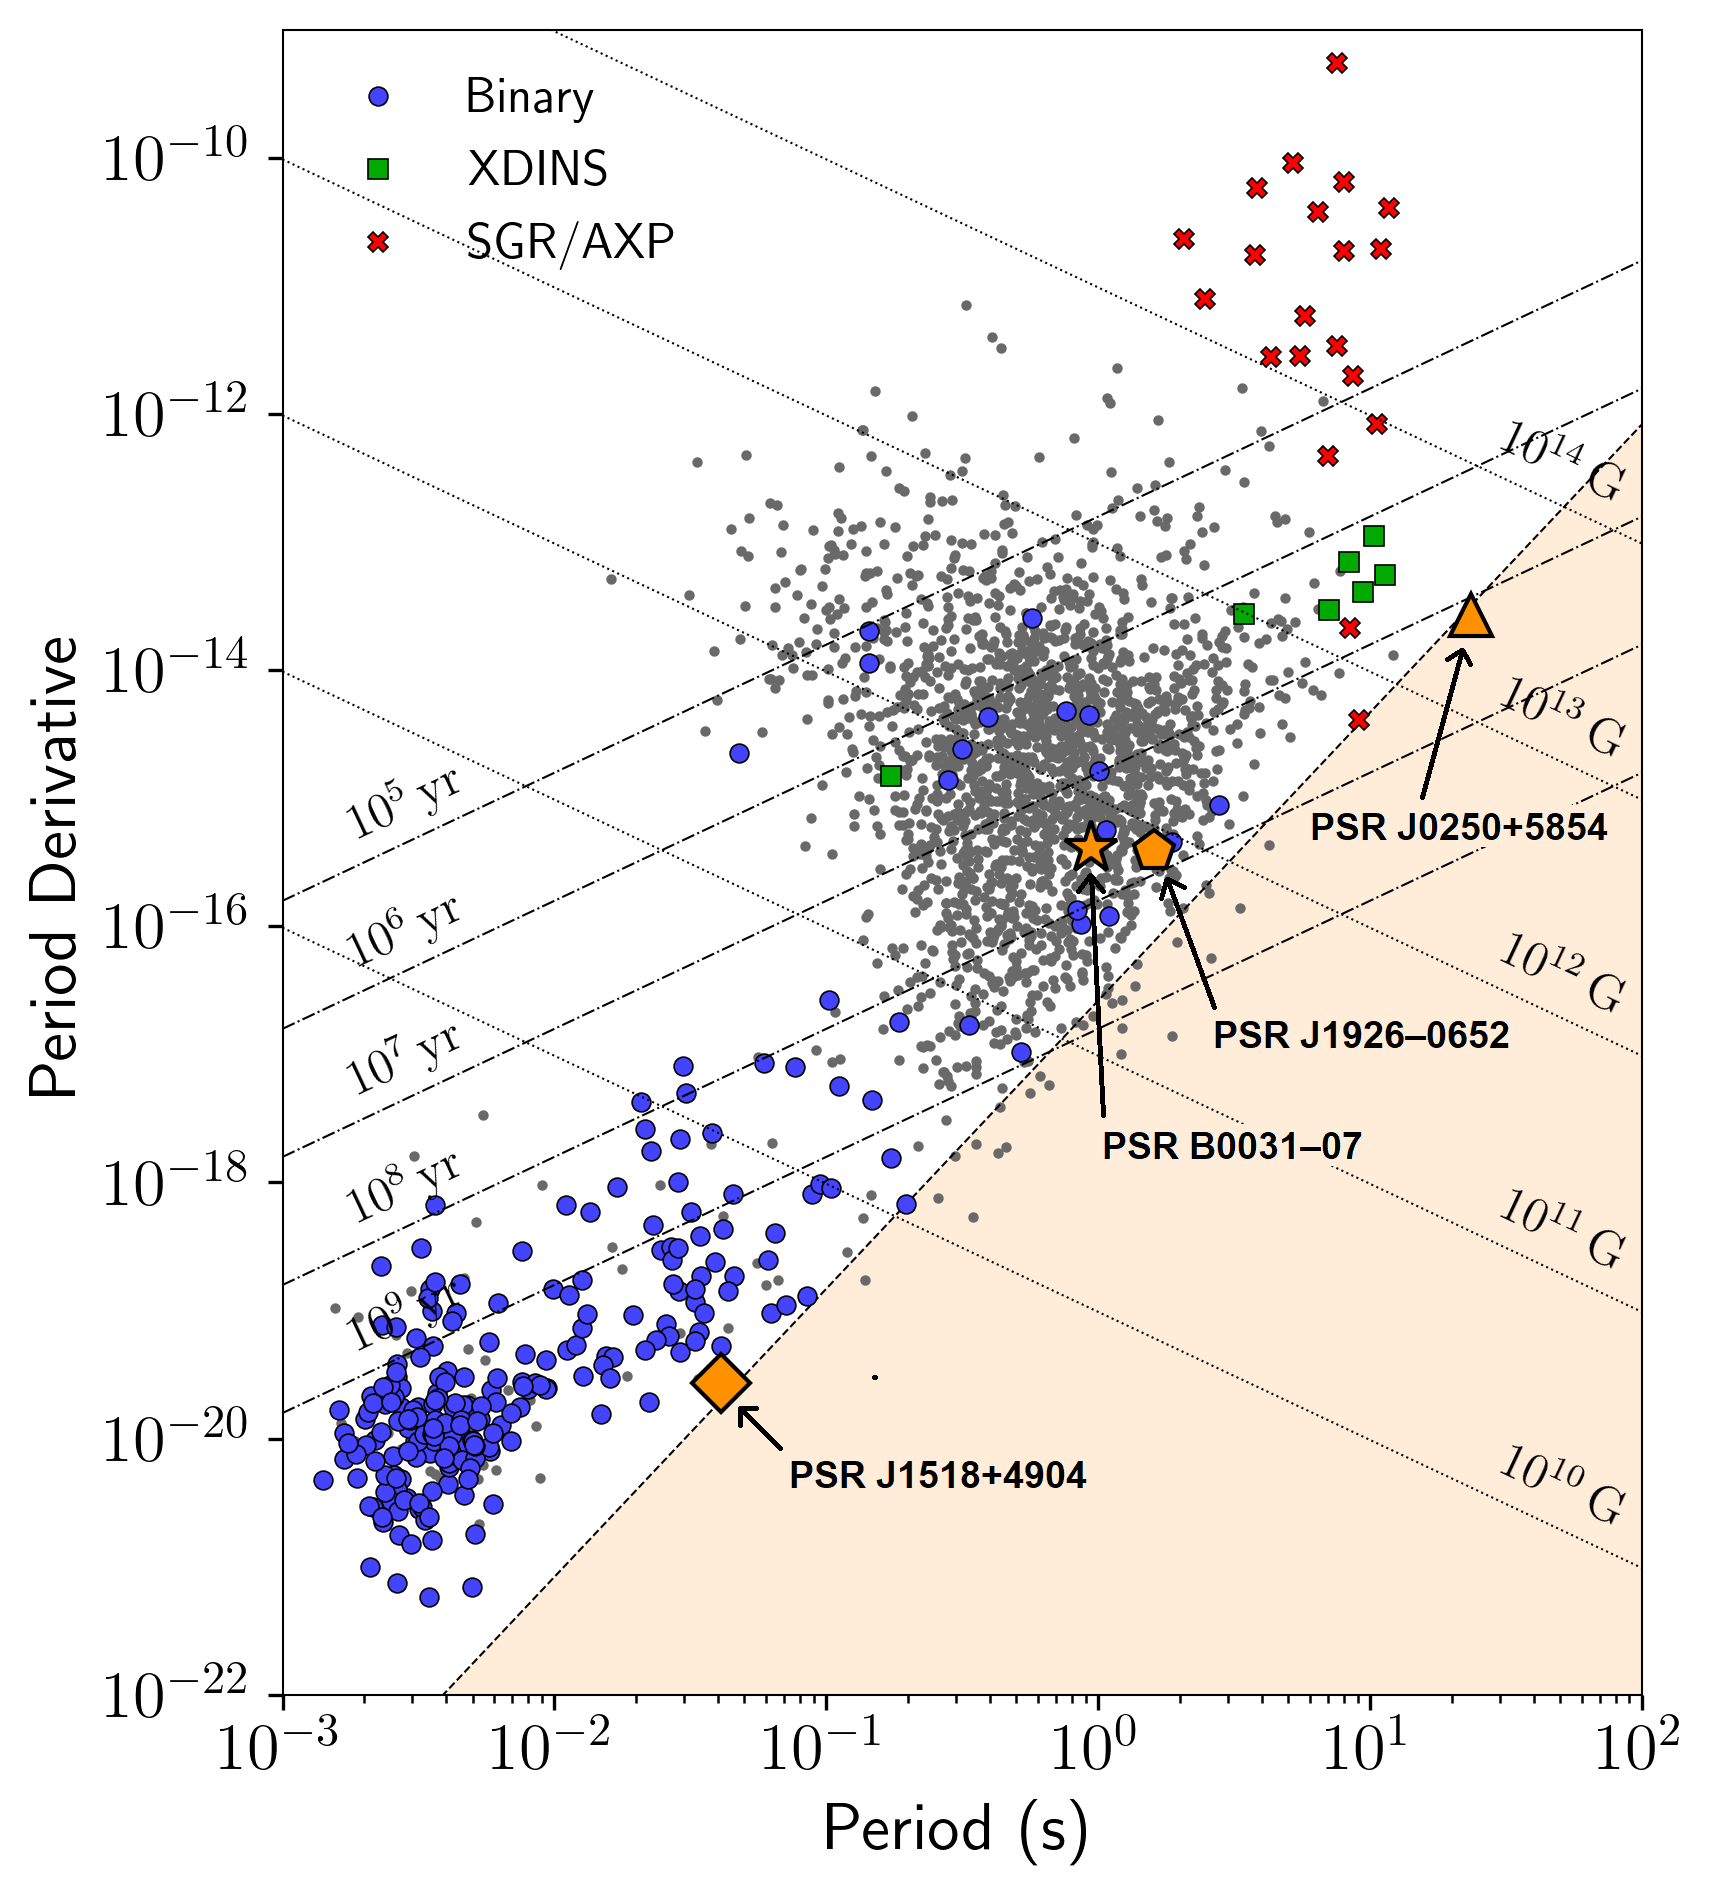
\includegraphics[width=1.0\textwidth]{Figures/Introduction/ppdot_diagram_labelled}
        \caption[The period/period derivative diagram]{The $P$-$\dot{P}$ diagram, showing the pulsar population with parameters retrieved from the ATNF pulsar database \citep{ATNFcatalogue} in May 2021. The blue circles indicate pulsars in a binary system. The red crosses show the magnetars, while the green squares highlight XDINSs. The four different orange shapes indicate PSRs~B0031$-$07 (star), J1926$-$0652 (pentagon), J1518+4904 (diamond), and J0250+5854 (triangle). The Python module \texttt{psrqpy} published by \citet{Pxxx2018} was used to create the diagram.}
        \label{fig: intro - ppdot diagram}
    \end{center}
\end{figure}
From the $P$-$\dot{P}$ diagram, groupings of pulsars can be identified, as discussed next.


\subsubsection*{``Normal'' pulsars}
\label{sec: intro - general intro - pulsar population - normal}

The majority of pulsars are found in the middle of the $P$-$\dot{P}$ diagram, and are often referred to as the ``normal'' pulsars. They typically have periods of around 0.5~s and spin-down rates of ${\sim}10^{-15}$~s~s$^{-1}$, giving them estimated magnetic fields of $B_s \sim 10^{11}--10^{13}$~gauss. Pulsars are thought to be born in the upper left of the $P$-$\dot{P}$ diagram with relatively short periods and high spin-down rates: as they age, they migrate towards the bottom right following a contour of constant $B_s$ if dipole radiation is the only rotational energy loss mechanism, although more complex evolutionary tracks have been theorised (see e.g. \citealt{JKxx2017} and references therein) until they cross the ``death line'', which is the theoretical limit below which it is believed that radio emission ceases to be produced. It is not a sharp limit however, and is sometimes referred to as more of a ``death valley''. The death line in Fig.~\ref{fig: intro - ppdot diagram} is the boundary of the pale yellow shaded region, and the model shown here is given by Eq.~6 of \citet{ZHMx2000}. It can be seen that a number of pulsars, including the slow pulsar PSR~J0250+5854 (see Chapter~\ref{chapt: J0250}), lie beyond this limit -- this highlights that this subject is a topic of much debate, and multiple different death line models have been proposed \citep[e.g.][]{CRxx1993,ZHMx2000, FKxx2006, JKxx2017, MBMA2020}.


\subsubsection*{Millisecond pulsars}
\label{sec: intro - general intro - pulsar population - MSPs}

Towards the lower left of the $P$-$\dot{P}$ diagram are the millisecond pulsars, or MSPs. These are much older pulsars with much lower spin-down rates of ${\sim}10^{-20}$~ss$^{-1}$. The majority of MSPs are in binary systems (indicated by the blue points in Fig.~\ref{fig: intro - ppdot diagram}), and are ``recycled pulsars''. These are old pulsars in binary systems who accrete matter from their companions. This transfers angular momentum to the pulsar, causing it to spin up to very short periods, and can also suppress their magnetic fields \citep{BKxx1974, SMSN1989}. Their short periods make MSPs ideal precision timing sources for the detection of gravitational waves, through pulsar timing arrays \citep[e.g][]{FBxx1990,MHB+2013}. At present only one binary MSP is known to have another pulsar as companion -- the ``double pulsar'', PSRs~J0737–3039A ($P=22.7$~ms) and J0737–3039B ($P=2.8$~s) discovered by \citet{BDP+2003}.

\subsubsection*{Magnetars and more}
\label{sec: intro - general intro - pulsar population - magnetars etc}

The most energetic pulsars can be found up in the top right of the $P$-$\dot{P}$ diagram. These include the magnetars (shown by the red crosses in Fig.~\ref{fig: intro - ppdot diagram}), given their name due to their extremely strong magnetic fields ($>10^{14}$~G). As of November 2020 there are 24 confirmed magnetars and 6 candidate sources\footnote{\url{http://www.physics.mcgill.ca/~pulsar/magnetar/main.html}} \citep{OKxx2014}. Magnetars produce mostly high energy emission, for example X-rays and $\gamma$-rays, and include the soft gamma repeaters (SGRs) which produce bursts of high energy emission at irregular intervals, and anomalous X-ray pulsars (AXPs) whose emission is believed to be produced by the decay of their magnetic fields \citep{TDxx1995, TDxx1996, Mxxx2008}. While most magnetars are only detected via their high energy emission, radio pulses have been detected from five: 1E~1547.0$-$5408 \citep{CRHR2007a}, PSR~J1622$-$4950 \citep{LBB+2010}, PSR~J1745$-$2900 \citep{EFK+2013}, XTE~J1810$-$197 \citep{CRH+2006}, and Swift~J1818$-$1607 \citep{ERB+2020, LSJB2020}.

One of the sources studied in this thesis (PSR~J0250+5854, the orange triangle in Fig.~\ref{fig: intro - ppdot diagram}, see Chapter~\ref{chapt: J0250}) lies close to a cluster of objects known as X-ray Dim Isolated Neutron Stars (XDINSs; indicated by the green squares). There are seven of these objects (informally known as ``The Magnificent Seven'', e.g. \citealt{Hxxx2007}) which are characterised by pulsed X-ray emission with a soft, blackbody-like spectrum and periods between 3.4 to 11.3 seconds. Although they are similar to and potentially evolved from magnetars \citep{VRP+2013}, no radio emission from XDINSs has been detected \citep{Jxxx2003, KKM+2003, KML+2009}.









\section{Radio emission and models}
\label{sec: intro - emission models}

% Briefly summarise the emission models, and stress that this thesis is particularly interested in the single pulse and polarisation properties
Based on the work by \citet{Gxxx1968}, who first suggested that pulsars are magnetised, rotating neutron stars, \citet{GJxx1969} investigated the simplest case of a pulsar in which the magnetic dipole axis is aligned with the rotation axis. They concluded that, despite the intense surface gravitational field, the pulsar must possess a dense magnetosphere which co-rotates with the star up until the light cylinder radius (see Fig.~\ref{fig: intro - basic geometry}). In the corotating plasma, the net magnetospheric charge density is $7\times10^4 B_z P^{-1}$ electronic charges per cubic metre, where $B_z$ is the component of the magnetic field in the direction of the rotation axis ($B_z = \mathbf{B}\cdot\mathbf{\hat{\Omega}}$, measured in gauss) -- this is known as the Goldreich-Julian density, $\rho_\mathrm{GJ}$, and is the net charge density required to screen the rotation-induced electric fields \citep{GJxx1969}.

Magnetic field lines which exit the light cylinder do not re-enter, instead closing in a boundary zone layer near the shell of the supernova remnant. Charged particles can escape the pulsar along these open field lines forming the wind zone surrounding the light cylinder, up to a distance of about one tenth of the radius of the supernova remnant shell surrounding the star. Here, unlike closer to the star, the currents due to the charged particles are the main source of the magnetic field. It is the motion of the charged particles along the open field lines within the light cylinder which gives rise to the beamed electromagnetic radiation from the magnetic poles.

Further analysis by \citet{RSxx1975} led to one of the best-known models of pulsar radio emission. % Nuclei -- mostly iron -- in the crust of neutron stars form a tightly bound condensed state due to the strong magnetic field: both theory and observations have shown that the surface of a pulsar is not hot enough to sustain an ejection of positive ions to balance the outflow of electrons along the open field lines. This is true for all but the youngest (most energetic) and hottest of pulsars, for example the Crab \citep{RSxx1975}.
Like \citet{GJxx1969}, \citet{RSxx1975} considered an aligned rotator; one in which the magnetic moment is antiparallel to the spin angular momentum vector (in the community this is sometimes referred to simply as a pulsar, whereas the opposite case where the magnetic and spin vectors point in the same direction is called an ``anti-pulsar''). By assuming that ejected electrons do not return to the star by the open field lines, they concluded the existence of a ``polar gap'' in the magnetosphere, reaching from the stellar surface to an altitude of around 100~metres. Within the gap, $\mathbf{E}\cdot\mathbf{B} \neq 0$, although it essentially vanishes elsewhere -- this leads to a large potential difference across the gap of around $10^{12}$~V. On microsecond timescales the gap breaks down by forming electron-positron pairs; the positrons move outward along the open field lines and the electrons flow back to the surface to close the homopolar generator circuit.

Also in the related \citet{Sxxx1971} model, electron-positron pairs are produced from the energetic curvature radiation photons from accelerating charges travelling along the curved field lines. The charge density along the open field lines was taken to be much less than required for co-rotation \citet{GJxx1969}, essentially treating the open field line region as empty of corotating magnetosphere. In this scenario \citet{RSxx1975} argue that the potential different in the gap would much greater than the space charge effects in the magnetosphere associated with bringing the electrons to relativistic speed. If the gap is not present and acceleration of the electrons is purely due to space charges, for a pulsar with $P\approx1$~s there would be a potential drop of less than $10^{10}$~V above the surface \citep{Mxxx1974}, far too low for further pair production by curvature radiation. \citet{RSxx1975} therefore conclude that the polar gap is a crucial part of pulsar radiation and that the magnetosphere within the open field lines also plays an important role, an idea that has been developed in more recent years \citep[e.g.][]{CRxx1980,ZQHx1997a,Txxx2010, SMGx2015}.

\citet{RSxx1975} also predicted that the breakdown of the polar gap occurs through discrete, localised ``sparks'' which inject positron beams into the magnetosphere beyond the gap. There, they produce the plasma and bunching that ultimately leads to the production of coherent radio emission. As discussed in Sec.~\ref{sec: intro - emission models - single pulse phenomena - carousel model}, the location of the sparks on the polar cap determines the pattern of sub-beams which rotate in a carousel-like structure, which can explain the existence of so-called drifting subpulses.



\subsection{Polarisation properties}
\label{sec: intro - emission models - polarisation}

Radio waves are a form of electromagnetic (EM) radiation, which in a vacuum is a transverse wave. The magnetic and electric field components are perpendicular to one another, both being orthogonal to the direction of propagation of the wave. The orientation of the electric field vector determines the polarisation state of the EM wave.

A common representation of polarisation is by the use of Stokes' parameters -- $I$, $Q$, $U$, and $V$ -- which fully describe the average polarisation state of a beam of light. The total intensity of the beam is given by $I$, which for a fully-polarised beam is the combination under quadrature of the other components:
\begin{equation}
    \label{eq: stokes parameters quadrature}
    I^2 = Q^2 + U^2 + V^2.   
\end{equation}
The Stokes parameters are formed by considering the combination of the two (Cartesian) components of the electric field of the EM wave, $E_x$ and $E_y$. By time-averaging the $x$ and $y$ components of a crossed dipole common in the ``linear feed'' of many receivers, the Stokes parameters can be written
\begin{align}
    I = \langle E_x^2 \rangle + \langle E_y^2 \rangle \label{eq: intro - stokes I linear}\\
    Q = \langle E_x^2 \rangle - \langle E_y^2 \rangle \label{eq: intro - stokes Q linear}\\
    U = 2\langle E_x\rangle \langle E_y\rangle \cos\phi \label{eq: intro - stokes U linear}\\
    V = 2\langle E_x\rangle \langle E_y \rangle \sin\phi \label{eq: intro - stokes V linear}
\end{align}  
where $\phi$ is the relative phase between $E_x$ and $E_y$ \citep{Handbook}.

Linear polarisation is represented by the orthogonal components $Q$ and $U$, where the total linearly-polarised intensity of a wave is given by $L = \sqrt{Q^2 + U^2}$. The circularly-polarised intensity $V$ can be either positive or negative depending on the handedness of the circular polarisation, and occurs when there is a phase delay between the $x$- and $y$-components of the electric field vector. The polarisation vector $\mathbf{p}$, expressed in Cartesian coordinate as $(Q,U,V)$, has a magnitude
\begin{equation}
    \label{eq: polarisation vector magnitude}
    |\mathbf{p}| = \sqrt{Q^2 + U^2 + V^2}
\end{equation}
and can be smaller than $I$ for partially polarised radiation.

The polarisation vector is commonly depicted by use of the Poincar\'e sphere, as illustrated in Fig.~\ref{fig: intro - Poincare sphere}. This graphically represents the orientation of the polarisation, and the polarised intensity corresponds to the radius of a sphere. The space is defined by three orthogonal bases: $\hat{\mathbf{Q}}$, $\hat{\mathbf{U}}$, and $\hat{\mathbf{V}}$. Figure~\ref{fig: intro - Poincare sphere} also introduces the position angle (PA) $\psi$ of the linear polarisation and the ellipticity angle $\chi$. As indicated in the figure, the PA is given by
\begin{equation}
    \label{eq: position angle definition}
    \psi = \frac{1}{2}\arctan\bigg(\frac{U}{Q}\bigg),
\end{equation}
and the ellipticity angle is 
\begin{equation}
    \label{eq: ellipticity angle definition}
    \psi = \frac{1}{2}\arctan\bigg(\frac{V}{\sqrt{Q^2 + U^2}}\bigg) = \frac{1}{2}\arctan\bigg(\frac{V}{L}\bigg).
\end{equation}
The double angles $2\psi$ and $2\chi$ in Fig.~\ref{fig: intro - Poincare sphere} highlight the fact that the angles of polarisation are periodic on $\pi$ rather than $2\pi$ for phase. The PA is of particular interest in pulsar astronomy as it varies as function of pulse longitude, describing a characteristic S-shaped curve, which can be interpreted by the Rotating Vector Model as will be described next.
\begin{figure}
    \begin{center}
        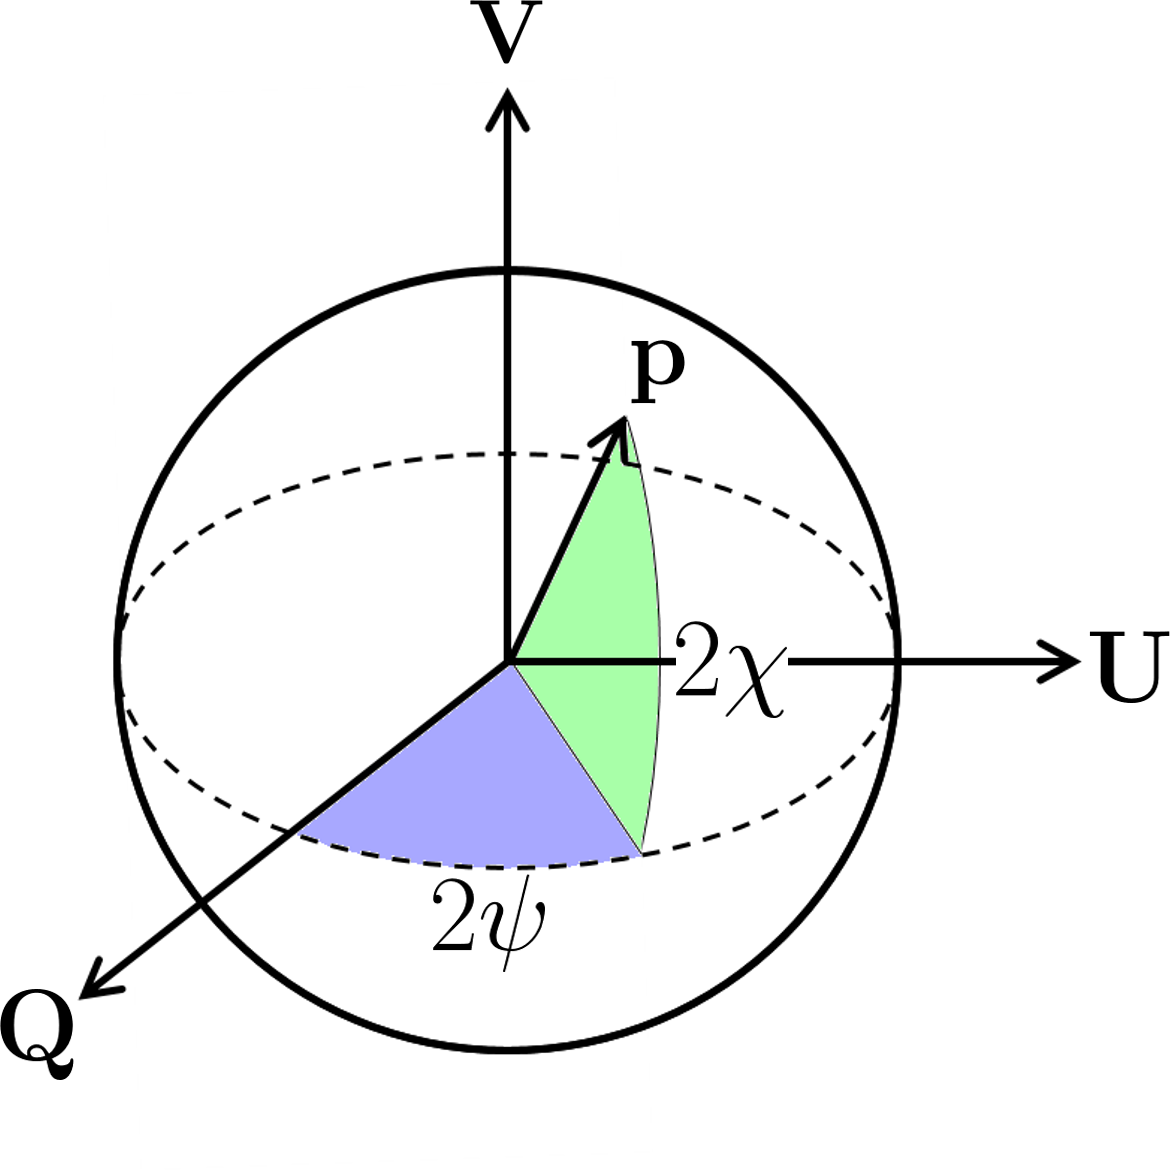
\includegraphics[width=0.4\textwidth]{Figures/Introduction/poincare_sphere}
        \caption[Polarisation vector on the Poincar\'e sphere]{A representation of the polarisation vector $\mathbf{p}$ on the Poincar\'e sphere. The mutually-orthogonal basis vectors are formed by Stokes parameters $Q$, $U$, and $V$. The position angle is given by $\psi$, whilst the ellipticity angle is $\chi$. If a wave is purely linearly polarised, then $\mathbf{p}$ will lie in the $(Q,U)$ plane.}
        \label{fig: intro - Poincare sphere}
    \end{center}
\end{figure}

\subsubsection*{Linear polarisation and the Rotating Vector Model}
\label{sec: intro - emission models - polarisation - RVM}

% Describe expectations (strong linear polarisation)
The emission of radio pulsars, especially the younger ones, typically exhibits a high degree of polarisation, especially linear polarisation \citep[e.g.][]{QMLG1995, CMKx2001}. The position angle of the linear polarisation (PA) is observed to depend on pulse longitude, and hence is often associated with the changing orientation of the magnetic field lines with respect to the observer's line of sight. This is illustrated in Fig.~\ref{fig: intro - vela polarisation}, which shows the polarised profile of the Vela pulsar (PSR~B0833$-$45). The shape of the PA curve is usually simple, S-shaped, and monotonic, even when the total intensity profile has multiple components \citep{WCL+1999}. This implies that the orientation of the linear polarisation is independent of the intensity of different sources of emission, affected only by the location of source within the emission region.
\begin{figure}
    \begin{center}
        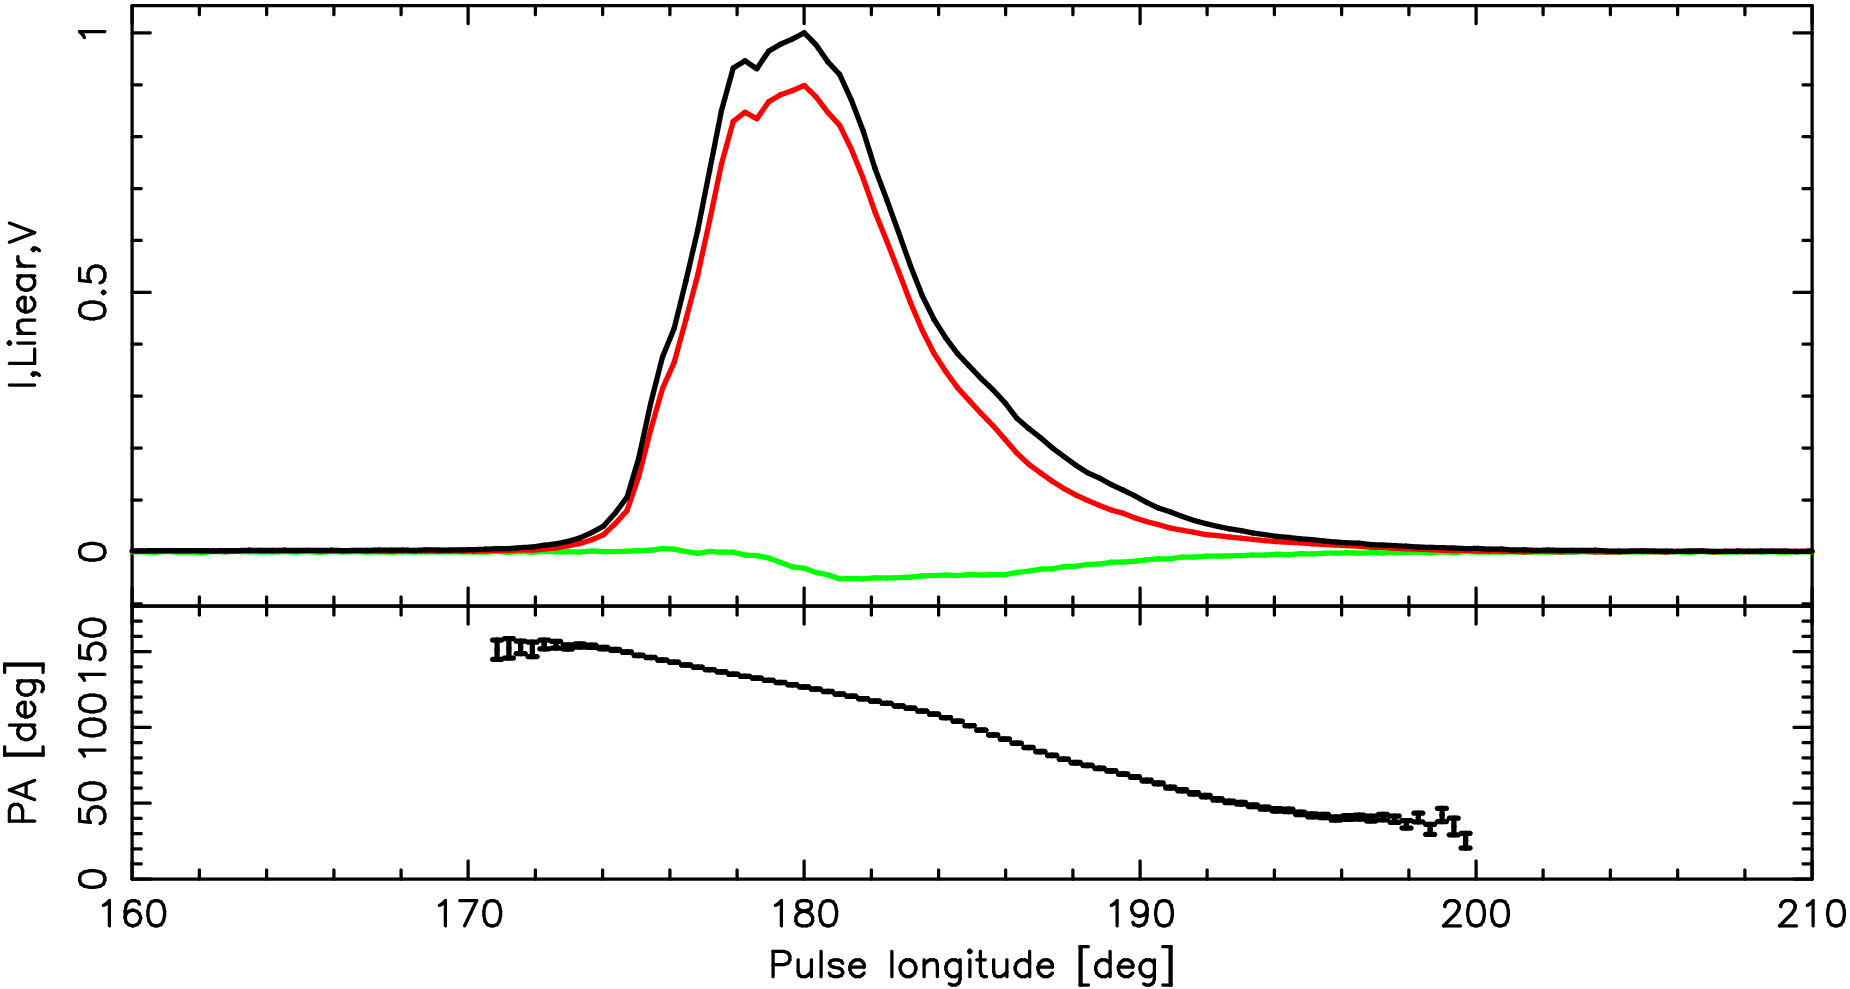
\includegraphics[width=0.8\textwidth]{Figures/Introduction/vela.png}
        \caption[The polarisation properties of the Vela pulsar]{The highly polarised profile of the Vela pulsar (PSR~B0833$-$45) at 1375~MHz. The upper panel shows the total intensity profile, linear polarisation, and circular polarisation by the black, red, and green lines respectively. The lower panel shows the PA of the linear polarisation, illustrating how it varies smoothly as a function of pulse longitude. This data was was recorded by \citet{KJxx2006}, and is publicly available from the European Pulsar Network Database\footnotemark.}
        \label{fig: intro - vela polarisation}
    \end{center}
\end{figure}

\footnotetext{\url{http://www.epta.eu.org/epndb/}}\citet{RCxx1969} showed that the PA curve can be fitted well by a very simple, geometric model: the Rotating Vector Model (RVM). The RVM is built upon the following assumptions: first, each magnetic field line lies in a single plane containing the magnetic axis (as would be the case for a static, dipolar magnetic field). This plane defines the orientation of linear polarisation of any radiation emitted from the vicinity of this field line \citep[e.g.][]{Cxxx2015}. From the point of view of an observer looking down on the star, the magnetic field lines surrounding the pole would appear radially-projected. As the line-of-sight traverses this area, the angle of the observed field line changes smoothly, by up to $180\degr$. This is illustrated in Fig.~\ref{fig: intro - RVM field line schematic}.
\begin{figure}
    \begin{center}
        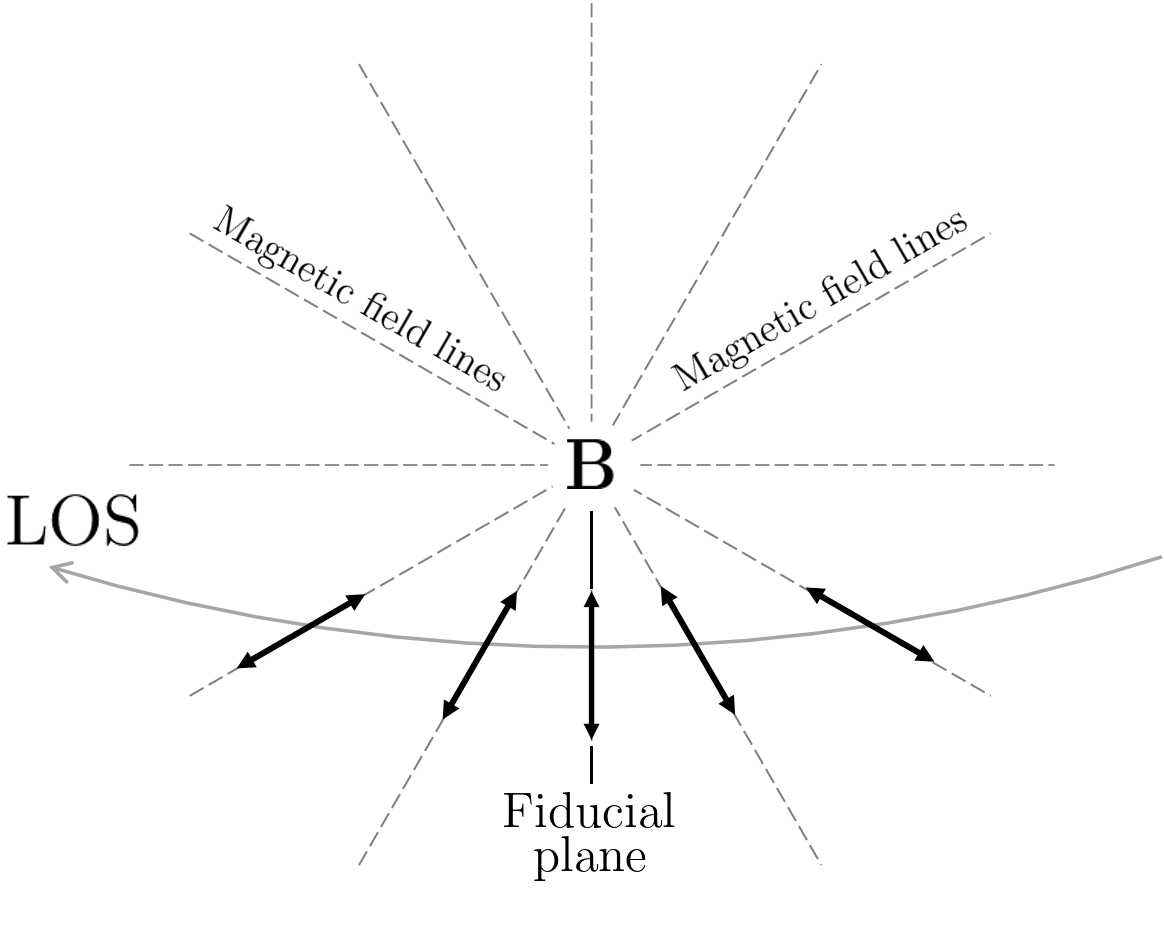
\includegraphics[width=0.75\textwidth]{Figures/Introduction/PA_curve_illustration}
        \caption[How the local magnetic field direction determines the PA as the pulsar rotates]{An illustration of the change in orientation of the magnetic field lines seen by the observer as the line of sight passes over them. The orientation of the field lines defines the direction of linear polarisation of the radio emission (thick black arrows), which changes smoothly as a function of pulse longitude.}
        \label{fig: intro - RVM field line schematic}
    \end{center}
\end{figure}
The shape of the PA curve and the RVM depends on the viewing geometry of the star, $\alpha$ and $\beta$. \citet{Kxxx1970} showed that the change of PA, $\psi$, as a function of pulse longitude, $\phi$, can be described by 
\begin{equation}
    \label{eq: intro - RVM}
        \tan(\psi - \psi_0) = \frac{\sin(\phi-\phi_0)\sin\alpha}{\sin(\alpha+\beta)\cos\alpha-\cos(\alpha+\beta)\sin\alpha\cos(\phi-\phi_0)},
\end{equation}
which describes a monotonic, S-shaped curve with an inflection point at ($\phi_0$, $\psi_0$). The maximum rate of change of the PA occurs when the observer's line of sight crosses the fiducial plane formed between the magnetic and rotation axes,
\begin{equation}
    \label{eq: intro - RVM gradient}
    \dphi{\psi}\bigg|_{\phi=\phi_0} = \frac{\sin\alpha}{\sin\beta}.
\end{equation}
Since the inclination angle $\alpha$ is constrained to lie between $0\degr$ and $180\degr$, $\sin\alpha$ is always positive, and therefore the sign of Eq.~\eqref{eq: intro - RVM gradient} depends only on the sign of $\beta$. In principle, fitting Eq.~\eqref{eq: intro - RVM} to the observed PA as a function of pulse longitude of a given pulsar can be used to determine the geometry, $\alpha$ and $\beta$ \citep[e.g.][]{EWxx2001, JWxx2006,RWJx2015a}. However, often the PA curve is only observed for a small faction of a full rotation of the start (limited by the ``duty cycle'' of the pulses), and only its steepest gradient is well constrained. This necessitates further constraints to be applied using other methods. This is explored for the newly discovered pulsar J1926$-$0652 in Chapter~\ref{chapt: J1926}, and for the slow pulsar PSR~J0250+5854 in Chapter~\ref{chapt: J0250}.

Equation~\eqref{eq: intro - RVM gradient} suggests that the inflection point of the RVM curve should occur at the same pulse longitude as the fiducial plane of the total intensity pulse profile, $\phi_\mathrm{fid}$. However, observations show a small delay: $\Delta\phi = \phi_0 - \phi_\mathrm{fid}$. \citet{BCWx1991} modelled this delay as arising from relativistic aberration and retardation effects, and showed that it is dependent on the emission height $h_\mathrm{em}$
\begin{equation}
    \label{eq: intro - BCW shift}
    \Delta\phi = \frac{8\pi h_\mathrm{em}}{cP} = \frac{4h_\mathrm{em}}{R_\mathrm{LC}}.
\end{equation}

\subsubsection*{Orthogonal polarisation modes}
\label{sec: intro - emission models - polarisation - OPMs}

Many pulsars, especially younger, more energetic pulsars, have PA curves that can be closely modelled by the RVM. 
However, some pulsars are observed which show a rapid change in PA as a function of pulse longitude, of approximately $90\degr$. 
Early studies of Arecibo polarisation data by \citet{RCBx1974} and  \citet{BRCx1976} suggested the existence of two nearly orthogonal emission modes which change in relative intensity across the profile.
These competing polarisation modes distort the ``fundamental'' RVM curve, causing a rapid transition between states: when the dominant mode changes, a jump in the average PA occurs. This can be seen for example in the integrated profile of PSR~J0742$-$2822 as shown in Figure \ref{fig: intro - J0742 OPMs}.
\begin{figure}
    \begin{center}
        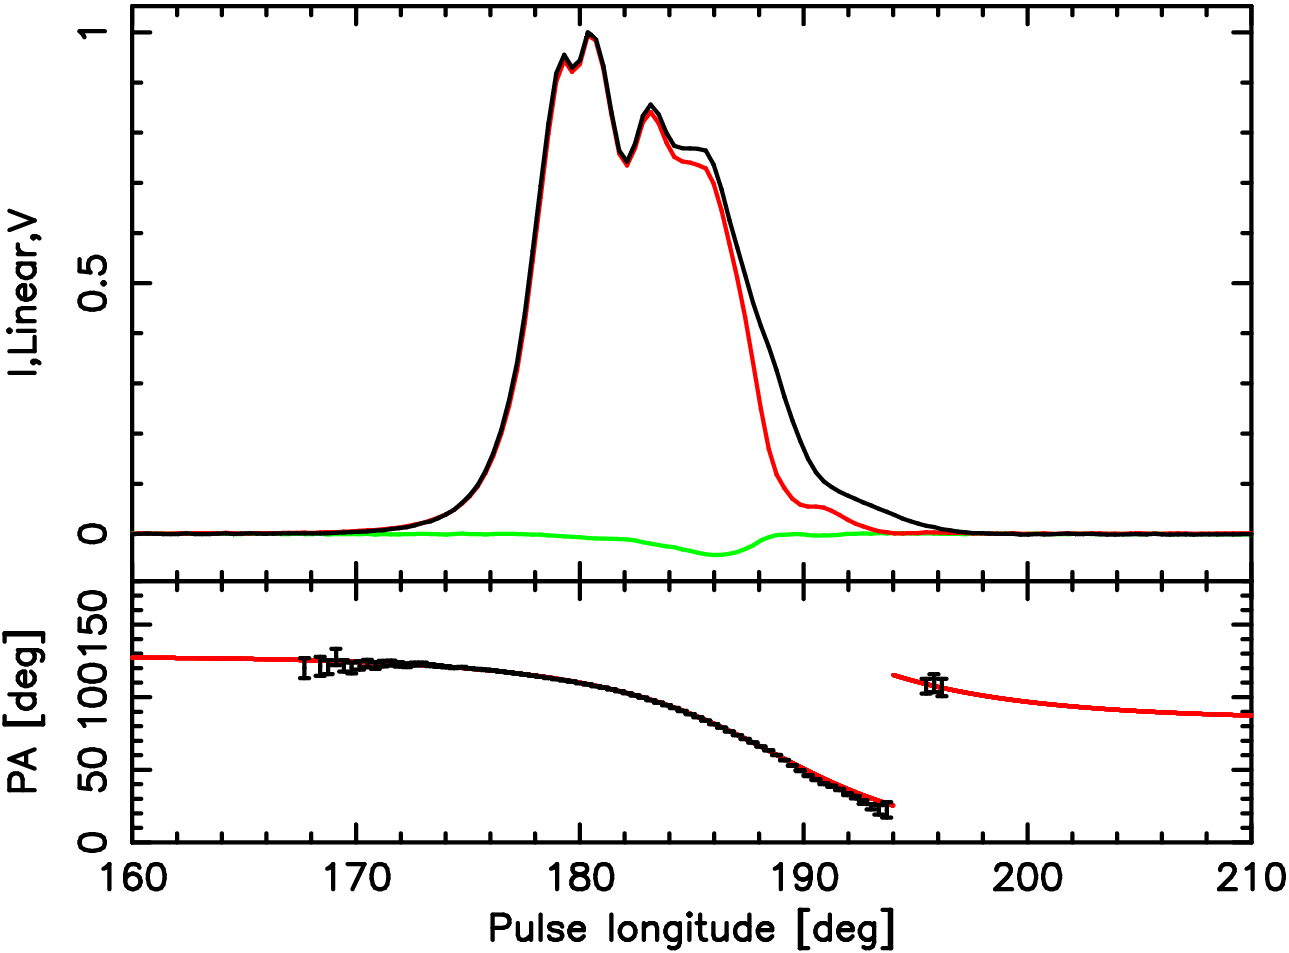
\includegraphics[width=0.6\textwidth]{Figures/Introduction/opm_profile}
        \caption[Orthogonal polarisation modes in PSR~J0742$-$2822]{The profile of PSR~J0742$-$2822 at a wavelength of 20~cm as observed by \citet{RWJx2015a}. In the upper panel total intensity is shown in black, linearly polarised intensity in red, circular polarisation in green. The lower panel shows the position angle as a function of pulse longitude, and the red line is the best-fitting RVM curve. An orthogonal mode transition can be seen at around pulse longitude $195\degr$. }
        \label{fig: intro - J0742 OPMs}
    \end{center}
\end{figure}

\citet{MSxx2000} showed that the two modes can exist simultaneously, but in general the intensity ratio between them depends on pulse longitude. When the two modes are viewed simultaneously, the subsequent incoherent mixing of the orthogonal polarisations means that the resulting observed signal becomes depolarised. This reinforces the suggestion that the emission is intrinsically highly polarised \citep[e.g.][]{BRxx1980,SCR+1984, MSxx1998}. A possible explanation for the origin of OPMs was given by \citet{Mxxx1979} and \citet{ABxx1986}, who proposed that the distinct modes are caused by the difference in ray paths of natural modes in plasma. Waves in an ultra-relativistic plasma propagate via two modes; the ``ordinary'' (O-) mode, and the ``extraordinary'' (X-) mode, which are orthogonal. In the presence of a strong magnetic field, such as is found in pulsar magnetospheres, the X-mode decouples from the plasma and propagates freely. However, the O-mode remains connected to the plasma and is therefore subject to refraction. The result is that the O-mode radiation follows a curved path whilst the X-mode follows a shorter, straight path from the point of emission. Although they may originate from the same location, the path length difference and curvature of the path means that an observer will see the two modes with different delays, giving the impression of two orthogonally polarised images of the same emission structure.

\subsubsection*{Polarisation conventions in pulsar astronomy}
\label{sec: intro - emission models - polarisation - conventions}

Throughout this work, it has been very important to define reference frames and conventions for the various coordinate systems encountered. A large part of this thesis deals with polarisation data, and it is therefore prudent to discuss the coordinate systems and conventions used in pulsar astronomy. In 1969, the Institute of Electrical and Electronics Engineers (IEEE) defined a right-handed coordinate system for the propagation of radio waves \citep[][still valid as of 2019]{IEEE1969}. In this system the x-axis points towards the North and the y-axis points East (as projected onto the plane of the sky for an earthbound observer), whilst the z-axis extends towards the observer. The position angle of linear polarisation (PA; $\psi$) increases from the North towards the East, so \textit{anticlockwise} from the observer's perspective. This coordinate system is shown in Fig.~\ref{fig: intro - IEEE polarisation frame}.
\begin{figure}
    \begin{center}
        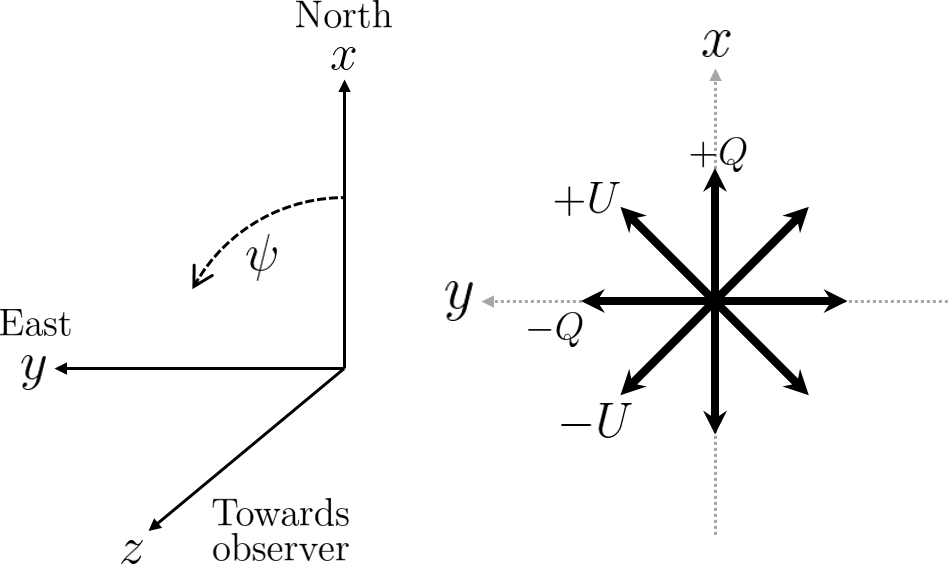
\includegraphics[width=0.6\textwidth]{Figures/Introduction/IEEE_coordinate_system}
        \caption[Reference frame of IEEE polarisation conventions]{The IEEE coordinate system which defines the position angle of linear polarisation ($\psi$) on the sky from the perspective of an Earth-bound observer (left). The right-hand panel shows the coordinate system that defines the linear Stokes parameters $U$ and $U$. $+Q$ lies along the $x$-axis, while $-Q$ lies on the $y$-axis. $+U$ is oriented at $45\degr$ between the two. }
        \label{fig: intro - IEEE polarisation frame}
    \end{center}
\end{figure}
For right-handed circular polarisation, the PA of the electric field vector increases with time, forming a left-handed helix -- this implies that the x-component of the field lead the y-component. In this coordinate system, the linear Stokes parameters $Q,U$ are uniquely defined: positive $Q$ lies along the x-axis whilst negative $Q$ lies along the y-axis. Positive $U$ lies along the line $y=x$, where $\psi=\pi / 4$ \citep{HBxx1996}. The International Astronomical Union (IAU) adopted this definition \citep{IAU1974}, supplementing it with a definition of the sign of Stokes $V$: positive for right-handed circular polarisation \citep{Wxxx1973,TMSx1986}.

However, the early pulsar observations \citep[e.g.][]{Mxxx1971} established a convention in which Stokes $V$ is positive for left-handed circular polarisation as defined by the IEEE; opposite to that of the IAU convention. This alternate definition is the convention described by \citet{Kxxx1966} and is that used by the \textsc{psrchive} software package and encoded in the \textsc{psrfits} file format \citep{SMJR2010}. The consequences of discrepancy between the geometry of the RVM and the IEEE polarisation convention were explored by \citet{EWxx2001}. They note that $\alpha$ and $\beta$ are both defined as increasing away from the positive spin axis of the pulsar, which points in the direction of the angular momentum vector (i.e. the North pole). This means that in the framework of the RVM as given by Eq.~\eqref{eq: intro - RVM} \citep{Kxxx1970}, the position angle $\psi$ is defined as increasing in the \textit{clockwise} direction (this was also pointed out by \citealt{DTxx1992} and \citealt{APTW1996}). The required correction to previously published geometries is $\alpha = 180\degr - \alpha_\mathrm{RVM}$ and $\beta = -\beta_\mathrm{RVM}$, where the subscript denotes values measured by fitting the RVM \citep{EWxx2001}. This correction is highlighted where relevant in this thesis. \todo{MAKE SURE IT IS! C12 AND 0250}


\subsection{Single pulse phenomena}
\label{sec: intro - emission models - single pulse phenomena}

% Observation of drifting subpulses
The integrated pulse profile is characteristic and unique to each pulsar, and is typically stable and reproducible over many hundreds of pulse periods. However, it often hides a number of interesting features which vary on timescales comparable to $P$. The individual pulses of most radio pulsar are made up of several components, which are typically between one and three degrees in width, much narrower than the full profile width which spans the \textit{pulse window} typically covering around $10\degr$ in pulse longitude \citep[e.g.][]{KWJ+1994}. These components, known as ``subpulses'' can behave in different ways: they may appear at random locations within the pulse window; they may favour certain longitudes, consistently appearing in the same place in different pulses; or they may steadily drift across the pulse window at a roughly constant rate. This last case is the phenomenon of \textit{drifting subpulses}, which are believed to occur in more than 55~per~cent of pulsars \citep{WESx2007}, and is a feature of great interest in this thesis.

Drifting subpulses were first noted by \citet{DCxx1968} in pulsars CP~1919+21 and AP~2015+28, and define two more important periodicities. The spacing between subpulses within a given pulse is labelled $P_2$, whilst the number of pulses it takes for a particular pattern of subpulses to repeat is labelled $P_3$ \citep{SSPW1970} -- these quantities are illustrated in Fig.~\ref{fig: intro - drifting subpulses}. In this nomenclature, the pulsar rotation period $P$ is also called $P_1$ \citep{Bxxx1973}, a convention used in this thesis hereafter. Figure~\ref{fig: intro - drifting subpulses} shows a ``pulse stack'', created by splitting the time-series data into blocks of length equal to one stellar rotation period, so each block contains a single pulse. The individual pulses are typically stacked as shown, with the pulse number (i.e. time) increasing vertically upwards. This allows systematic deviations in pulse profile shape to be identified easily -- if drifting subpulses are present, they will form diagonal bands in the pulse stack, referred to as ``driftbands'.'  
\begin{figure}
	\centering
	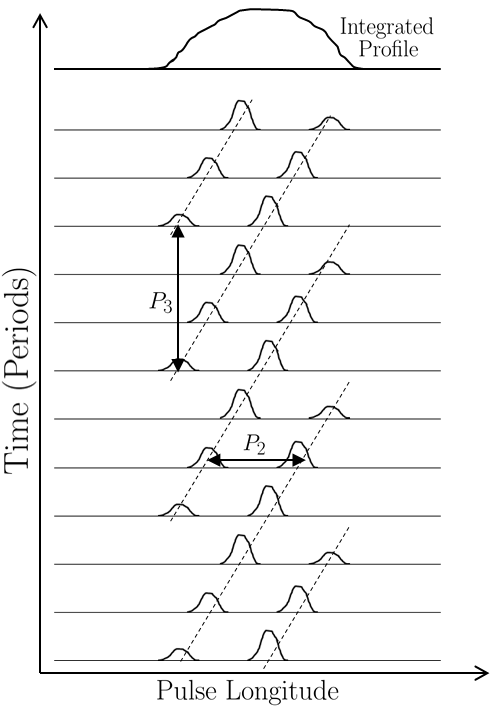
\includegraphics[width=0.4\textwidth]{Figures/Introduction/drifting_subpulses}
    \caption[Drifting subpulses and the definitions of $P_2$ and $P_3$]{An illustration of drifting subpulses showing the periods $P_2$ and $P_3$, where $P_2$ is the spacing between successive subpulses and $P_3$ is the spacing between driftbands (indicated by dotted lines). The top of the plot shows the integrated profile \citep[after][]{Bxxx1973}.}
    \label{fig: intro - drifting subpulses} 
\end{figure}

Some pulsars exhibit an abrupt cessation of emission within a single period. Known as ``nulling'', this was first reported by \citet{Bxxx1970b} and is now believed to be a relatively common feature, seen in approximately 8~per~cent of the population \citep[e.g.][]{Rxxx1976, Bxxx1992, LWxx1995,  WMJx2007, GJKx2012, SMxx2021}. The length of null has been seen to vary significantly across the population, from several periods to days, months, or even years.  The portion of time that a pulsar is nulling is referred to as its ``nulling fraction'' and varies from near zero (PSR~B1737+13, \citealt{Bxxx1992}) to over 90~per~cent (PSR~B1713$-$40, \citealt{WMJx2007}). Nulling is believed to be an extreme form of profile ``mode switching'', where the pulsar has two or more distinct stable profile shapes. This was first observed in PSR B1237+25 by \citep{Bxxx1970b} and largely affects the normal, longer period pulsars, although it has also been reported in the MSPs \citep[e.g][]{KLL+1999,MKMP2018, BMRx2019}. If the pulsar shows drifting subpulses, a mode-switch may be associated with a change in the drifting behaviour. PSR~B0031$-$07 is one such pulsar that is explored in detail in Chapter~\ref{chapt: B0031}. This pulsar has three distinct drift modes with $P_3 \approx 12 P_1$, $P_3 \approx 7 P_1$, and $P_3 \approx 4 P_1$ \citep{HTTx1970, VKxx1997,SMKx2005, SMS+2007, MBT+2017,MBW+2019}.





\subsubsection*{The carousel model}
\label{sec: intro - emission models - single pulse phenomena - carousel model}

The drifting subpulse phenomenon can be attributed to the breakdown of the strong electric field in the polar gap through localised ``sparks''. These sparks are the sites of pair production, creating the bunches of particles that are accelerated by the fields and give rise to coherent radio emission in sub-beams in the open field line region \citep{RSxx1975, CRxx1977, Bxxx1982, FRxx1982,GSxx2000}. Under the action of $\mathbf{E} \times \mathbf{B}$ drift, these sparks complete one full circulation around the magnetic axis in a period $P_4$.  If the circulation time is slow, then $P_4 = NP_3$, where $N$ is the number of sub-beams. The carousel is believed to circulate in the same direction as, but slightly slower than, the pulsar spins. If the number of sub-beams is high, or the circulation speed is rapid, this can lead to aliasing. Aliasing in the context of the rotating carousel describes a stroboscopic effect whereby a quickly circulating carousel, sampled one each stellar rotation ($P_1$) would appear to be moving much slower than it actually is, potentially even appearing to move in the opposite direction. More details on the effects of aliasing are given in Appendix~\ref{app: geometry derivations}. The classical picture of the carousel beam structure is shown in Fig.~\ref{fig: intro - carousel schematic} and consists of multiple evenly spaced sub-beams arranged on the polar cap in one or more nested cones.
\begin{figure}
	\centering
	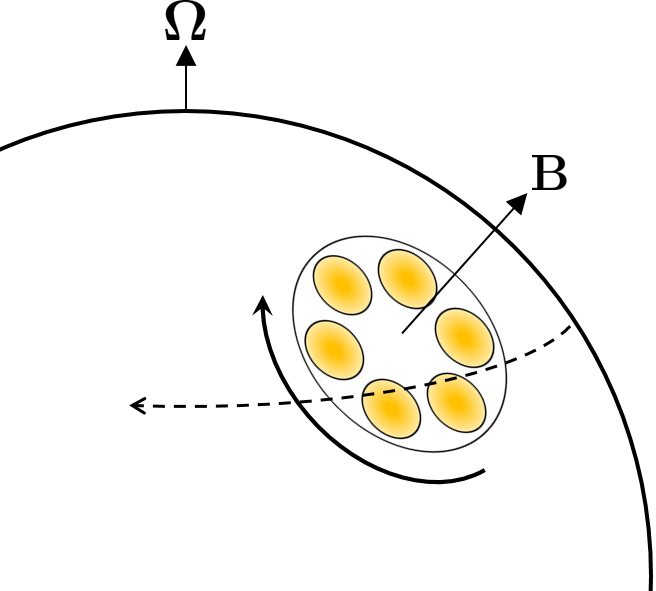
\includegraphics[width=0.5\textwidth]{Figures/Introduction/carousel_schematic}
    \caption[Drifting subpulses and the definitions of $P_2$ and $P_3$]{An illustration of a carousel of sparks circulating around the magnetic pole in the polar cap. As the carousel circulates, the observer's line of sight (dashed line) passes over different sub-beams at different times.}
    \label{fig: intro - carousel schematic} 
\end{figure}
As well as drifting subpulses \citep[e.g.][]{GSxx2000,GMxx2001,WESx2006,WSEx2007}, the carousel model is able to explain many other observed phenomena. ``Bidrifting'' pulsars, which show simultaneous drifting in opposite directions, can be explained by elliptical carousels \citep{QLZ+2004, Wxxx2016, WWxx2017, SLxx2017, SLWM2020} and periodic nulling can be explained by the extinguishing of one or more sub-beams as the carousel circulates, giving rise to nulls that last an integer multiple of $P_3$ cycles \citep{HRxx2007, HRxx2009, RWxx2008}.

In order to gain a clearer understanding of the physics of the carousel, it is useful to recreate an image of it. By considering the path the footprint of the observer's line of sight takes through the emission region \citet{DRxx1999} defined a cartographic transform to map the observed intensity at a certain pulse longitude in a given pulse to a position on the polar cap. In Appendix~\ref{app geometry derivations} I show how this transform is derived from first principles, and extend it to the case of short circulation times where aliasing is occurring, and also demonstrate how it may be applied to data folded at the period $P_3$ (see Sec.~\ref{sec: intro - emission models - single pulse phenomena - P3 folding}). 

\citet{DRxx2001} used this transform to study the structure of PSR~B0943 in two different drift modes -- the ``bright'' (B) mode and the ``quiescent'' (Q) mode -- at 430~MHz. This pulsar has an average $P_3 = 11.1 P_1$, although the authors argue aliasing is taking place. They made an image of the B mode carousel with 20 sparks, and a circulation time $P_4 = 37 P_1$, and the Q mode was also compatible with this structure. Their multi-frequency analysis revealed a similarity of the sub-beams at different frequencies, and suggested that the radiation is produced from columns of plasma, which in turn implies the existence of some form of ``seeding'' mechanism at the stellar surface. The authors argue that the sub-beam emission is therefore bound neither to the magnetic field, nor the stellar surface.

\subsubsection*{Subpulse polarisation}
\label{sec: intro - emission models - single pulse phenomena - subpulse polarisation}

Compared to the integrated pulse profile, individual pulses exhibit a higher degree of polarisation \citep[see][]{PulsarAstronomy}. This is to be expected since the polarisation vector $\mathbf{p}$ varies somewhat between pulses, and vector addition of many will therefore lead to depolarisation. \citet{THHM1971} examined the subpulses of PSR~B0809+74 and found that the successive drifting bands display almost identical polarisation behaviour, having a high degree of linear polarisation and showing a systematic PA swing with a negative gradient through each subpulse. The PA at the leading edge of each subpulse was approximately the same, as was its rate of change, such that all subpulses showed roughly the same position angle near their peaks. A small amount of circular polarisation was visible near the centre of each pulse window. \citet{RRS+2002} argued that the linear polarisation angles of the drifting subpulses are oriented according to the stellar magnetic field. Furthermore, they showed that the subpulses of PSR~B0809+74 contain two orthogonal modes of polarisation (OPMs) which arise from emission directed either parallel or perpendicular to the magnetic field lines. They find that the OPM transitions occur at progressively earlier phases in successive pulses, remaining almost parallel to the driftbands and therefore at the same position within subpulses as they drift across the pulse window. This was what was observed by \citet{THHM1971}, albeit somewhat smeared. The two modes gradually mix across the profile window as subpulses at the edges tend to show only one of the modes. The sign of the circular polarisation is closely correlated with the power of the two linear modes, while being slightly displaced in pulse longitude.

\citet{RRL+2006} expanded the analysis of PSR~B0809+74, attempting to map the emission region surrounding the magnetic pole, using the cartographic transforms of \citet[][see Appendix~\ref{app: geometry derivations}]{DRxx2001}. They found two possible configurations of the carousel: 8 to 10 sub-beams for an ``outer'' (equatorward) traverse of the line-of-sight (LOS), and 25 to 40 sub-beams for an ``inner'' (poleward) traverse. They found that one OPM is strongly associated with the overall intensity pattern, forming roughly azimuthally symmetric patches on the inner edge of the observed emission (limited by the fact that the minimum approach of the LOS to the magnetic axis is $\beta$ and therefore some emission is never seen). In contrast, the other OPM is radially extended and is strongest between the total power beamlets. The authors did not attempt to provide a physical explanation for the observed structure, but did note that the azimuthal and radial offset between modes is as expected from an earlier independent analysis of polarised conal profiles \citep{RRxx2003}. This OPM behaviour could potentially be explained by the O- and X-mode propagation introduced in Sec.~\ref{sec: intro - emission models - polarisation - OPMs}, in which the two modes would be offset images of the same carousel.



\subsubsection{$P_3$-folding}
\label{sec: intro - emission models - single pulse phenomena - P3 folding}

\todo{INSERT NICE FULL PAGE FIGURE SOMEWHERE HERE THAT SHOWS HOW THE BEAM MAP (CAROUSEL) LEADS TO A PULSE STACK, AND HOW THAT MAY THEN BE FOLDED TO CREATE A HIGH S/N P3 FOLD. USE B0809 DATA?}

In order to more clearly see the shape of driftbands the technique of ``$P_3$ folding'' can be used. In this method the data is averaged over the modulation cycle to produce an image of the average driftband, with a higher signal-to-noise ratio than for the individual driftbands, permitting detailed studies of the average drifting behaviour. This technique, while seeming simple in principle, can be complicated by the fact that the $P_3$ periodicity is rarely stable, often fluctuating somewhat about a mean value over the course of an observation. If such data were naively folded with a fixed period, the variations can cause smearing of the driftband (see \citealt{DRxx2001} and \citealt{LKR+2002} for example). However, a method to do $P_3$ folding whilst taking into account these variations was first used by \citet{HSW+2013} to study PSR~B0809+74, which exhibits a somewhat variable $P_3$. This method is implemented in the \textsc{psrsalsa}\footnote{\url{https://github.com/weltevrede/psrsalsa}} suite of programs \citep{Wxxx2016} used throughout the work in this thesis, and works in the following way.

First, the rough $P_3$ value of interest is identified, typically using Fourier techniques such as the longitude-resolved fluctuation spectrum (LRFS; see Chapter~\ref{chapt: J1926}). The pulse stack is then divided into blocks of some integer multiple of $P_3$; $n\times P_3$. For example, if $P_3 = 12.6 P_1$, one might choose a block length of 38 pulses which encloses $ 3\times P_3$. When dividing the pulse stack care should be taken to ensure the blocks form continuous pulse sequences (i.e. nulls and mode changes are removed). Each block is then folded with a fixed period $P_3$. This initial crude folding increases the signal-to-noise (S/N) ratio of the drift bands within the block, which is beneficial when performing the cross-correlations as described below. On the other hand, if the $P_3$ variation timescales are short, then this fixed-period folding can lead to smearing, so some care must be taken in the choice of $n$. In practice, different block lengths are tried to visually judge the optimum compromise. Variations in $P_3$ are taken into account by cross-correlating the folded blocks by allowing an offset in pulse number before stacking them. This is an iterative process: the output from the first iteration is taken as a template for the next iteration, where the blocks are correlated with the template in order to determine their offsets. The benefit of this method is that the template will have a higher S/N ratio than the individual blocks, so alignment is more reliable after the initial pass. The rate of improvement decreases with subsequent iterations, so the number of iterations is chosen such that further processing would not significantly improve the results.


\section{Observation processing}
\label{sec: intro - observation processing}

To properly study the properties of radio pulsars, the observations must first be calibrated, and corrections made for a number of propagation effects. Both flux density calibration and polarisation calibration are commonly performed on the raw recorded data, and frequency-dependent effects such as dispersion and Faraday rotation must be removed in order to study the \textit{intrinsic} properties of the emission.

\subsection{Polarisation calibration}
\label{sec: intro - observation processing - polarisation calibration}

Pulsar polarisation can provide a wealth of information on the underlying emission physics and the propagation through the interstellar medium (ISM), but first it must be properly calibrated. In general, the measured Stokes parameters will differ from the intrinsic Stokes parameters of the source for a variety of reasons, primarily related to the properties of the receiver and the observing system. A common type of receiver is a linear feed, which consists of a pair of crossed dipole antennas used to detect the orthogonal electric field components of the incoming signal, $E_x$ and $E_y$. From these quantities the four Stokes parameters can be calculated using Eqs.~\eqref{eq: intro - stokes I linear}--\eqref{eq: intro - stokes V linear}.

The Stokes parameters can be presented as a vector. The intrinsic Stokes vector is transformed to the observed (un-calibrated) Stokes vector by the Mueller matrix \citep{Mxxx1948}, a $4\times4$ real-valued matrix of which seven values are independent and describe the effect of the signal chain on $E_x$ and $E_y$. Calibrating the observing system determines the frequency-dependent Mueller matrix, allowing the intrinsic Stokes vector to be calculated. The first of the seven independent values is the overall gain of the system, and its calibration is known as flux calibration (see Sec.~\ref{sec: intro - observation processing - flux calibration}).

Four parameters are known as ``leakage'' parameters. These describe the situation where the signal attributed to one of the dipoles appears in the output from the other dipole, due to cross-coupling of the supposedly orthogonal elements. An example where, for an incident wave which is totally linearly polarised in the vertical direction, the horizontal dipole registers a signal. The leakage parameters are specific to a given receiver and signal chain, so are a relatively constant property of the system and do not need to be measured for individual observations. It is impossible to eliminate all leakage, although careful instrument design can minimise its effects \citep[e.g.][]{RTxx2018}. 

The remaining two parameters in the Mueller matrix are the differential gain and differential phase. The differential gain describes slight differences in the sensitivity and amplification of the two orthogonal polarisation signals, whilst the differential phase accounts for lag between the two channels (as a result of different cable lengths for example). These effects can be measured by performing a calibration observation just before, or after, the actual observation of the pulsar. The calibration observation should be a pointing to a position at least one beam width away from the source of interest, but close enough that the properties of the background radio emission are similar. During this pointing the signal from a ``noise diode'' is recorded -- this is a pulsed signal with a known strength and polarisation that is artificially injected into the signal chain. If it is injected equally into the two dipoles (i.e. at an effective orientation of $45\degr$), then it is known that the output signal should be pure Stokes $U$ (see Eqs.~\eqref{eq: intro - stokes I linear}--\eqref{eq: intro - stokes V linear}). Deviations from this pure signal allow the differential gain and phase to be calculated. 

Combined, the leakage parameters and the differential gain and phase form the ``receiver solution'' which can be applied to raw data in order to calibrate its polarisation properties. One final effect that, depending on the telescope, must be accounted for is the rotation of the feed with respect to the sky in long tracking observations. This effect, known as ``parallactic angle'' rotation, affects any `alt-azimuth' telescope unless the feed is rotated during the observation. This correction is to compensate for the changing orientation of the feed with respect to the sky. For example, the 19-beam receiver on the Five-hundred-metre Aperture Spherical Telescope (FAST) is designed to rotate to keep the orientation of the feed relative to the source fixed over the course of a tracking observation \citep[e.g.][]{JYG+2019}.


\subsection{Flux calibration}
\label{sec: intro - observation processing - flux calibration}

Knowing the absolute flux density of a pulsar is necessary for calculating its spectral index, and examining its frequency evolution (see for example the work on PSR~J0250+5854 in Chapter~\ref{chapt: J0250}).
The simplest way of calculating the flux density of a pulsar is to use the radiometer equation \citep{Dxxx1946}. This can be adapted to estimate the mean flux density $S_\mathrm{mean}$ of a pulsar from its pulse profile, based on its measured signal-to-noise ratio (S/N) and the parameters of the telescope used in the observation. As shown by \citet{Handbook} the mean flux density (in mJy) of a pulsar of period $P$ seconds, with an equivalent width\footnote{The equivalent width is equal to the area of the profile divided by the peak value \citep[e.g.][]{TMxx1975}} of $W$ seconds is given by
\begin{equation}
    \label{eq: intro - pulsar radiometer equation}
    S_\mathrm{mean} = \frac{(\mathrm{S/N}) \beta T_\mathrm{sys}}{G\sqrt{n_\mathrm{p}t_\mathrm{obs}\Delta f}}\sqrt{\frac{W}{P-W}}.
\end{equation}
Here, $t_\mathrm{obs}$ is the length of the observation in seconds, and $\Delta f$ is the frequency bandwidth in MHz. The performance parameters of the telescope and its receiver system are usually known, and are the system noise temperature $T_\mathrm{sys}$ (K), its gain $G$ (K~Jy$^{-1}$), and $n_\mathrm{p}$ is the number of polarisation signals (for a single dipole $n_\mathrm{p} = 1$, or if two orthogonal polarisations are combined $n_\mathrm{p} = 2$). A small correction factor $\beta \gtrsim 1$ is included to account for digitisation losses and other slight imperfections in the signal chain, but is typically practically 1. The telescope performance parameters are usually available in technical publications: for example, the 19-beam receiver on FAST has a bandwidth of 400~MHz, $T_\mathrm{sys} \sim 19 - 27$~K, and $G\sim 11.5 - 16.0$~K~Jy$^{-1}$ \citep{JTH+2020}.

% Flux calibration using a reference source
Another method of performing flux calibration is to observe a calibration source with stable, known properties (i.e. its spectral index and flux density at a given frequency). This is done either before or after observing the pulsar of interest, and the a calibration source that is close to the pulsar should be chosen, in order to ensure that the background emission has similar properties. This allows the scale of the arbitrary ``machine units'' in which the data is recorded to be calculated, and the frequency response of the receiver to be determined. A noise diode can also be used in a similar fashion if its antenna noise temperature $T_\mathrm{cal}$ is known -- in this case, the noise diode can be pulsed synchronously with the pulsar such that both signals appear side by side. The pulsar signal can then be directly compared to the calibration signal. This is the system used on the Effelsberg telescope \citep{SGG+1995}.







\subsection{Effects of the interstellar medium}
\label{sec: intro - observation processing - ISM effects}

Pulsar radio signals are broadband, made up of a continuous spectrum of frequencies. As a signal propagates through the cold plasma of the interstellar medium (ISM), it is subject to effects such as scattering and dispersion. Linearly polarised signals will also be affected by Faraday rotation. Observations of radio pulsars can be used to infer both the dispersion measure and the rotation measure along a particular line of sight, which allow the properties of the interstellar medium to be modelled.

\subsubsection{Dispersion}
\label{sec: intro - observation processing - ISM effects - dispersion}

Dispersion is a property of EM wave propagation caused by the dependence of a wave packet's group velocity $v_\mathrm{g}$ on its frequency, $\nu$: in a cold, ionised plasma $v_\mathrm{g} = c\mu$, where $c$ is the speed of light in a vacuum, and $\mu$ is the refractive index of the medium through which it is travelling \citep{Handbook}. The ISM, being a cold plasma, has a refractive index of 
\begin{equation}
    \label{eq: intro - ISM refractive index}
    \mu = \sqrt{1-\bigg(\frac{\nu_\mathrm{p}}{\nu}\bigg)^2},
\end{equation}
where $\nu_\mathrm{p}$ is the plasma frequency, dependent on the density of electrons $n_\mathrm{e}$ in the ISM. Since $\mu < 1$ here, $v_\mathrm{g} < c$. A signal that travels a distance $d$ to reach an observer will be delayed by an interval
\begin{equation}
    \label{eq: intro - deispersive delay integral}
    \Delta t = \bigg( \int^d_0 \frac{\mathrm{d}l}{v_\mathrm{g}} \bigg) - \frac{d}{c}
\end{equation}
relative to a signal of infinite frequency (or a signal travelling through a vacuum), where the integral is along the line of sight.

Using an expression for the plasma frequency, Eq.~\ref{eq: intro - deispersive delay integral} is often parametrised in term of the \textit{dispersion measure} (DM) and the \textit{dispersion constant},  $\mathcal{D} = 4.148808(3)\times 10^3$~MHz$^2$~pc$^{-1}$~cm$^3$~s \citep{MTxx1972,Handbook}. The dispersive delay between two frequencies $\nu_1$ and $\nu_2$ (measured in MHz) is 
\begin{equation}
    \label{eq: intro - dispersive delay}
	\Delta t = \mathcal{D} \bigg(\frac{1}{\nu_1^2} - \frac{1}{\nu_2^2}\bigg) \times \mathrm{DM},
\end{equation}
where
\begin{equation}
    \label{eq: intro - dispersion measure definition}
	\mathrm{DM} = \int^d_0 n_\mathrm{e}\ \mathrm{d}l.
\end{equation}

The DM can be found by measuring the pulse arrival times as function of frequency. For an assumed model of electron density, such as NE2001 \citep{CLxx2002} or more recently YMW16 \citep{YMWx2016}, the distance to the pulsar can then be estimated by inverting Eq.~\eqref{eq: intro - dispersion measure definition}. If dispersion effects are not taking into account, the observed pulses will appear to be smeared as different frequencies within the observation bandwidth are delayed by different amounts, as illustrated in Fig.~\ref{fig: intro - DM illustration}. This is particularly true for wider bandwidth observations, and proper de-dispersion will yield higher resolution pulse profiles.
\begin{figure}
	\centering
	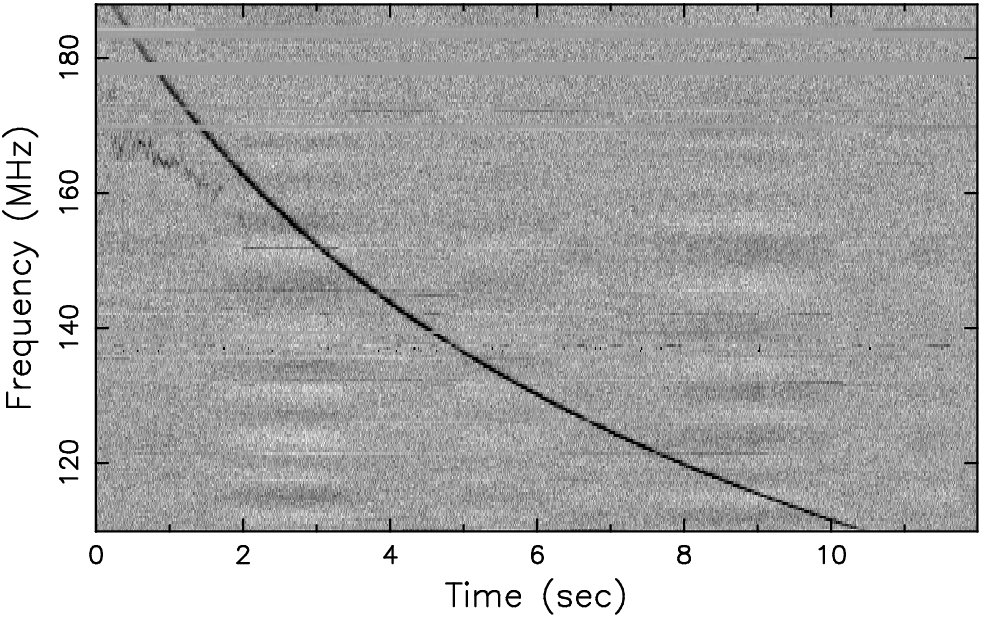
\includegraphics[width=0.6\textwidth]{Figures/Introduction/dispersed_data}
    \caption[The effect of dispersion on a pulse profile]{An illustration of the effect of dispersion on an observation of PSR~J0250+5854, which has a DM of 45.3~cm$^{-3}$~pc (see Chapter~\ref{chapt: J0250}). Lower frequencies arrive later than higher frequencies, giving the spectrum a characteristic sweep. Fitting the pulse arrival times as a function of frequency is used to find the DM through Eq.~\eqref{eq: intro - dispersive delay}.}
    \label{fig: intro - DM illustration} 
\end{figure}




\subsubsection{Scattering}
\label{sec: intro - observation processing - ISM effects - scattering}

Both scattering and scintillation are effects caused by inhomogeneities in the ISM. Scintillation causes frequency-dependent intensity variations of the source over time -- a familiar example of scintillation is the twinkling of stars, which is caused by turbulence in the atmosphere. Scattering is related to scintillation -- regions of different (electron) density in the ISM will refract emission, causing different rays to follow slightly different paths to an observer. These paths will have different lengths, and hence this results in a distribution of arrival times for a given pulse. The effect of this is to cause the pulse profile to broaden, forming a scattering tail.

The shape of a pulse due to scattering can be treated as the convolution of the intrinsic profile shape with a one-sided, exponential decay function of the form $\exp{(-t/\tau_\mathrm{s})}$ where $t$ is time and $\tau_\mathrm{s}$ is the characteristic scattering timescale \citep{Sxxx1968}. The scattering timescale is a frequency-dependent power law, i.e. $\tau_\mathrm{s} \propto \nu^{-\alpha}$, and the index $\alpha$ depends on the scattering model assumed. A commonly applied model is the ``thin screen'' model which treats all scattering as arising from a narrow region positioned half way between the pulsar and the observer \citep[e.g.][]{Sxxx1968, Wxxx1972}. This gives $4 < \alpha < 4.4$, where $\alpha = 4$ assumes Gaussian inhomogeneities \citep{Lxxx1971,LLxx1976} and $\alpha = 4.4$ assumes a Kolmogorov spectrum \citep{Rxxx1977,LRK+2015}. However, empirical fitting based on multi-frequency observations show that the scattering index varies across the pulsar population, spanning a range between 1.3 and 5.6 \citep{SDOx1980,LMG+2004, LDKK2013, LKKx2015, GKK+2017}. As well as frequency dependence, there is a correlation between the DM and $\tau_\mathrm{s}$ which has shown to be broadly parabolic in log-log space \citep[e.g.][]{BCC+2004,GKK+2017,IJWx2019}. This is likely due to the fact that pulsars with a higher DM are more distant, and hence their emission propagates through a greater depth of turbulent ISM. Overall, these relations imply that scatter broadening will be more significant at lower frequencies, and will more strongly affect distant pulsars with a higher DM.


\subsubsection{Faraday rotation}
\label{sec: intro - observation processing - ISM effects - faraday rotation}

A further frequency-dependent effect is Faraday rotation, which causes a change in the PA of linear polarisation of a signal. This can be described by a rotation in the $Q-U$ plane of the Poincar\'e sphere, determined by comparing the left- and right-hand circular polarisations of a beam of light. Compared to a wave of infinite frequency, the wave with frequency $\nu$ lags in phase $\Psi$ by
\begin{equation}
    \label{eq: intro - faraday rotation angle}
	\Delta\Psi_\mathrm{Faraday} = \int^d_0 (k_\mathrm{R}-k_\mathrm{L})\ \mathrm{d}l,
\end{equation}
here $k_\mathrm{R}$ and $k_\mathrm{L}$ are the wavenumbers of right- and left-hand circularly polarised light, and the integral is along the line of sight. Faraday rotation takes place in a cold, magnetised plasma with a wavenumber
\begin{equation}
    \label{eq: intro - magnetised plasma wavenumber}
    k(\nu) = \frac{2\pi}{c}\nu \sqrt{1-\bigg(\frac{\nu_\mathrm{p}}{\nu}\bigg)^2 \pm \frac{\nu_\mathrm{p}^2\nu_\mathrm{B}}{\nu^3} }.
\end{equation}
It can be seen that different directions of circularly polarised light propagate at different speeds: right-handed (`$+$') circularly polarised light travels faster than left-handed (`$-$') polarised light when $B_\parallel$ is positive, and vice versa when it is negative.
In Eq.~\eqref{eq: intro - magnetised plasma wavenumber} $\nu_\mathrm{B}$ is the cyclotron frequency which is governed by the strength of the Galactic magnetic field $B_\parallel$ along the line of sight,
\begin{equation}
    \label{eq: intro - cyclotron frequency}
	\nu_\mathrm{B} = \frac{eB_\parallel}{2\pi m_\mathrm{e}c}.
\end{equation}
In this relation $e$ and $m_\mathrm{e}$ are the electron charge and mass respectively. 

The change in the observed position angle PA $\psi$ by Faraday rotation is half the induced phase difference between the two circular polarisations, $\Delta\Psi_\mathrm{Faraday}$, and can be expressed in terms of the \textit{rotation measure} RM:
\begin{equation}
    \label{eq: intro - PA rotation angle}
	\Delta\psi_\mathrm{PA} = \frac{1}{2} \Delta\Psi_\mathrm{Faraday} \equiv \mathrm{RM} \times \lambda^2.
\end{equation}
In a similar manner to the dispersion measure, the rotation measure is defined by
\begin{equation}
    \label{eq: intro - rotation measure definition}
	\mathrm{RM} = \frac{e^3}{2\pi m_\mathrm{e}^2 c^4} \int^d_0 n_\mathrm{e}B_\parallel\ \mathrm{d}l .
\end{equation}

Faraday rotation manifests itself as a frequency-dependent rotation of the PA as illustrated in Fig.~\ref{fig: intro - RM illustration}.
\begin{figure}
	\centering
	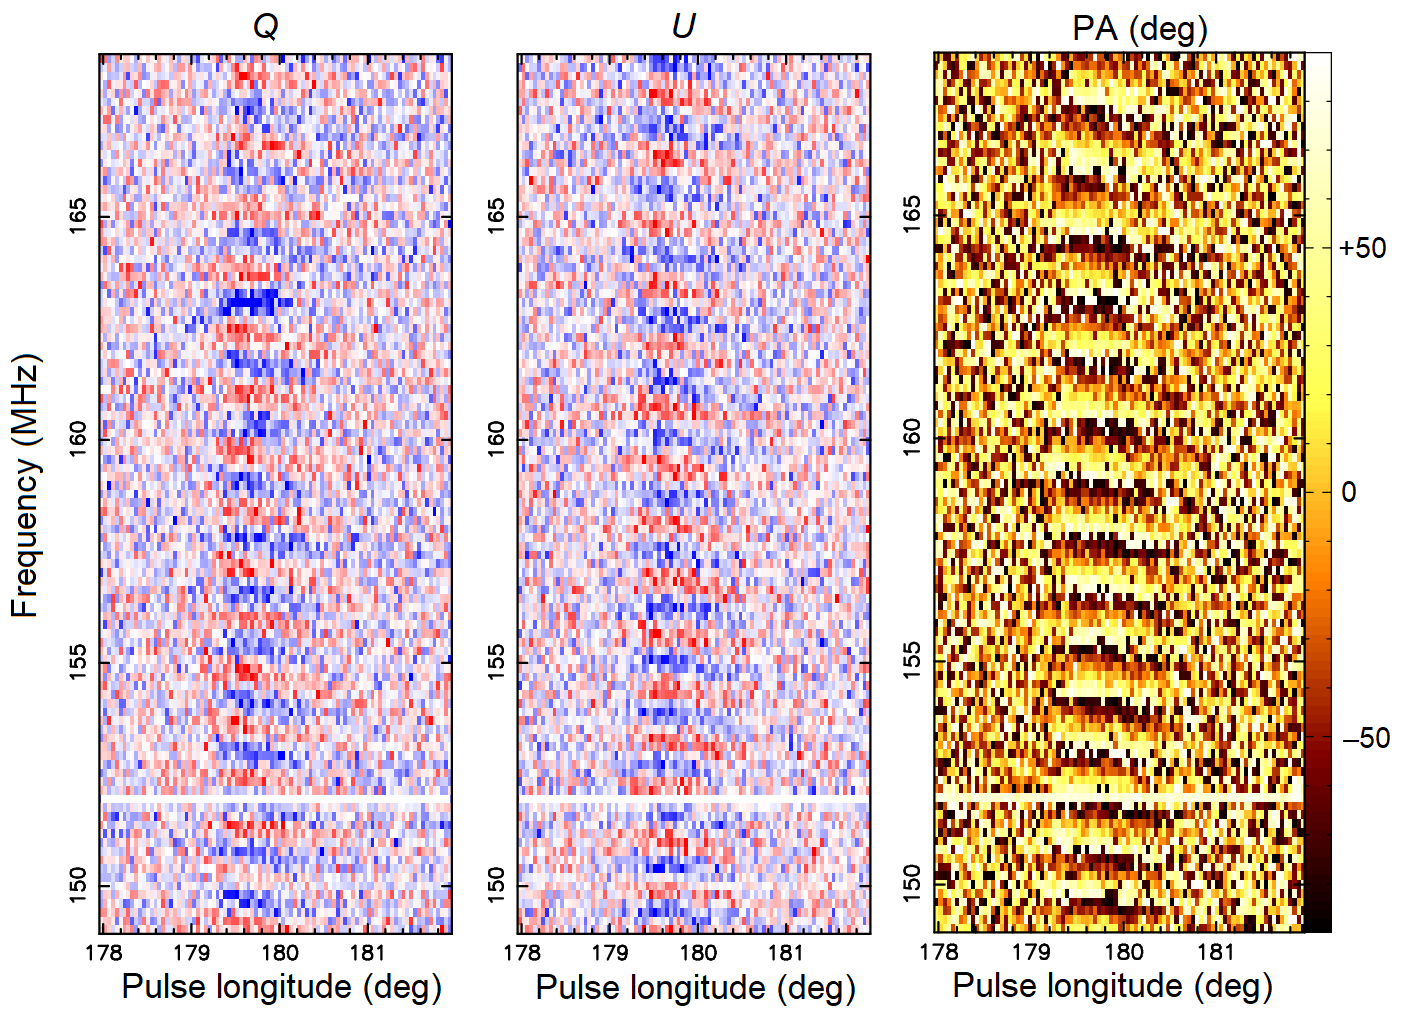
\includegraphics[width=0.8\textwidth]{Figures/Introduction/RM_data}
    \caption[The effect of Faraday rotation on polarisation]{An illustration of the effect of Faraday rotation on a polarised observation of PSR~J0250+5854, which has a RM of $-54.7$~rad~m$^{-2}$ (see Chapter~\ref{chapt: J0250}). There is a frequency-dependent rotation of the PA ($\psi$) which is stronger at lower frequencies. In Stokes $Q$ and $U$ this manifests as a variation between positive and negative values which can lead to apparent depolarisation if one sums over the frequency channels.}
    \label{fig: intro - RM illustration} 
\end{figure}
If uncorrected for it can lead to depolarisation if the frequency channels are summed over, meaning the linear polarisation will be underestimated and the sensitivity of the PA significantly reduced. De-Faraday rotation is the process of computing $\Delta\psi_\mathrm{PA}$ for each frequency channel according to Eq.~\eqref{eq: intro - PA rotation angle}, and then subtracting this phase from Stokes $Q$ and $U$. This requires the RM to be known.

A method to determine the RM in pulsar astronomy is the Fourier-based RM synthesis technique \citep{Bxxx1966, BBxx2005}, used to calculate the RM of PSR~J0250+5854 in Chapter~\ref{chapt: J0250} for example.
This method is based on calculating the RM power spectrum, $|F(\mathrm{RM})|^2$, using a discrete Fourier transform where 
\begin{equation}
    F(\mathrm{RM}) = K \sum_{j=1}^N P_j e^{-2i \mathrm{RM} (\lambda^2_j - \lambda^2_0)}.
\end{equation}
Here $K$ is a normalisation constant, $j$ is the frequency channel number (of which there are $N$), $P_j = Q_j + iU_j$ is the linear polarisation vector expressed as a complex number, $\lambda_j$ is the wavelength of channel $j$, and $\lambda_0$ is a reference wavelength (see \citealt{Hxxx2008} for further details). The RM power spectrum, $|F(\mathrm{RM})|^2$, which effectively quantifies the linear polarisation fraction as a function of trial RM, will peak at the RM of the pulsar. The power spectrum is usually taken to be the average across the pulse profile, however calculating the longitude-resolved RM can reveal slight deviations from the mean which point to magnetospheric effects taking place in the pulsar magnetosphere \citep{IJWx2019}.




















\section{Thesis outline}
\label{sec: intro - thesis outline}

This thesis focuses on two fields: investigations into the polarisation properties of radio pulsars, and the variability and systematic modulation of their individual pulses. The structure of the rest of this thesis is as follows.

Chapter~\ref{chapt: B0031} is an examination of the complex single-pulse polarisation behaviour of PSR~B0031$-$07, which exhibits both drifting subpulses and intensity-modulated orthogonal polarisation transitions. The complicated asymmetry in the drift modes is attributed to magnetospheric mixing of the OPMs, whilst the drifting subpulses are believed to originate from a carousel structure. This circulating carousel is mapped for the two drift modes observed and a model for the mixing of the OPMs is investigated.

Chapter~\ref{chapt: J1926} presents an investigation into PSR~J1926$-$0652, a pulsar with interesting single-pulse modulation properties discovered by the Five-hundred-metre Aperture Spherical Radio Telescope (FAST). Some of these results were published in \citet{ZLH+2019}. Polarised data from Parkes are also analysed in order to constrain the geometry of this pulsar. Alongside drifting subpulses, PSR~J1926$-$0652 shows frequent nulling, and strong evidence of a connection between the two mechanisms is found, with highly significant differences in the emission immediately prior to a null.

In Chapter~\ref{chapt: J1518} I present analysis of PSR~J1518+4904, which was observed four times with FAST in 2018 in order to study ``jitter noise'', stochastic variations in the profile shape on a pulse-to-pulse basis. Through Fourier analysis this pulsar was revealed to show very unusual single-pulse modulation, with multiple discrete $P_3$ periodicities present simultaneously at different pulse longitudes. A continuous, longitude dependence of $P_3$ was also observed for one of the profile components, which poses hard questions for current single-pulse modulation models.

Chapter~\ref{chapt: J0250} covers observations of the slowest known pulsar PSR~J0250+5854 \citep[$P_1 = 23.5$~s, ][]{TBC+2018} performed simultaneously with FAST and three Low Frequency Array (LOFAR) international stations. This new data increases the spectral coverage of this pulsar five-fold, and reveals that it has a steep spectrum with a low-frequency turnover. The profile is shown to broaden at higher frequencies, counter to expectations from radius to frequency mapping \citep[e.g.][]{KGxx2003}. Comparisons are drawn between this radio pulsar and the magnetars. This work is currently under review with Monthly Notices of the Royal Astronomical Society.


Finally, Chapter~\ref{chapt: conclusions} presents the conclusions of this work, including a summary of the remaining questions and suggestions for the potential direction of further research.